% \chapter{Notifications, tableaux de bord et reporting}
\glennchapter{CHAPITRE 7}{Notifications, tableaux de bord et reporting}
\vspace{1cm}
\markboth{Chapitre 7 : Notifications, tableaux de bord et reporting}{}
\label{chap:sprint3}
\addcontentsline{toc}{chapter}{Chapitre 7 : Notifications, tableaux de bord et reporting}
\setcounter{chapter}{7}
\setcounter{section}{0}

\localtableofcontents
\newpage
\pagebreak

\section*{Introduction}
\addcontentsline{toc}{section}{Introduction}

La préparation d'un prototype de gestion de parc informatique, dans le cadre de ce projet de fin d’études, ne saurait se limiter au stockage et à la manipulation des données. Elle exige également de fournir aux différents acteurs des instruments de pilotage permettant de suivre les défaillances, de mesurer des performances indicatives et de réagir aux événements critiques. C'est précisément l'ambition du troisième sprint, qui ajoute à la plateforme \textit{Parc Informatique FMM} une dimension décisionnelle et collaborative adaptée au contexte académique. Ce sprint introduit trois axes fonctionnels complémentaires. Le premier concerne la \textbf{notification en temps réel} : tout événement significatif — déclaration d'un incident, prise en charge par un technicien, résolution d'une panne — déclenche automatiquement une alerte push distribuée par Firebase Cloud Messaging (FCM), dans une version adaptée au cadre académique, à l'ensemble des utilisateurs disposant d'un jeton enregistré. Le deuxième axe porte sur les \textbf{tableaux de bord analytiques} : un composant de tableau de bord adaptatif restitue les indicateurs clés de performance (KPI), calculés dynamiquement à partir des données persistées en base MySQL, avec un contenu conditionné par le rôle de l'utilisateur authentifié. Le troisième axe couvre la \textbf{génération de rapports} : des documents PDF structurés retraçant les opérations de workflow (décharge, transfert, réforme d'équipements) et un export Excel de l'inventaire fonctionnel alimentent les processus d'audit et de planification de l'établissement.

L'architecture technique de ce sprint prolonge sans rupture la stack globale validée au Sprint 1. Les développements se concentrent donc sur l'enrichissement fonctionnel de cette base : notifications en temps réel, indicateurs analytiques et génération de rapports, tout en conservant une organisation cohérente avec les exigences opérationnelles du SmartLab de la Faculté de Médecine de Monastir.

% =========================================================
\section{Objectifs du Sprint 3}
\label{sec:objectifs_sprint3}

Les objectifs de ce sprint ont été définis en concertation avec les parties prenantes du projet — administrateurs du SmartLab, techniciens de maintenance et utilisateurs finaux — afin d'aligner les livrables sur les besoins réels de l'institution. Quatre grandes orientations structurent cette itération :

\begin{itemize}
    \item \textbf{Déploiement du canal de notification FCM :} intégrer Firebase Cloud Messaging dans le pipeline de traitement des événements métier afin de permettre une communication rapide et fiable entre le système et ses utilisateurs, indépendamment du support (navigateur de bureau, terminal mobile), dans une version adaptée au cadre académique ;

    \item \textbf{Conception et développement des tableaux de bord :} offrir à chaque profil d'utilisateur une interface de pilotage personnalisée, centralisant les indicateurs clés de performance et permettant une lecture rapide et efficace de l'état opérationnel du parc ;

    \item \textbf{Module de reporting et d'export :} permettre la génération à la demande de rapports d'activité structurés au format PDF ou Excel, consolidant les données historiques nécessaires aux audits et à la planification de la maintenance préventive ;

    \item \textbf{Optimisation des performances :} réduire les temps de réponse de l'API Express et améliorer la fluidité du rendu React, notamment pour les vues impliquant de grands volumes de données ou des calculs d'agrégation complexes.
\end{itemize}

\subsection*{Sprint Backlog}
\label{sec:sprint_backlog3}

Le tableau~\ref{tab:sprint_backlog3} consigne les tâches retenues pour ce sprint, leur niveau de priorité, l'estimation de la charge associée et les critères d'acceptation qui ont guidé la validation fonctionnelle.

\begin{table}[H]
    \centering
    \caption{Sprint Backlog — Sprint 3 : Notifications, tableaux de bord et reporting}
    \begin{tabular}{|p{4.8cm}|c|c|p{5.2cm}|}
        \hline
        \textbf{Tâche} & \textbf{Priorité} & \textbf{Charge (h)} & \textbf{Critères d'acceptation} \\ \hline
        Intégration Firebase FCM pour notifications push & Haute & 4 & Notification reçue dans les 2 s après l'événement déclencheur, en environnement local de développement \\ \hline
        Construction du tableau de bord multi-rôles & Haute & 12 & Tableau de bord accessible, KPI calculés dynamiquement, filtres fonctionnels \\ \hline
        Module de génération de rapports PDF/Excel & Haute & 6 & Rapport généré correctement, URL de téléchargement renvoyée \\ \hline
        Export CSV des statistiques & Haute & 3 & Fichier exporté sans perte de données, encodage UTF-8 respecté \\ \hline
        Optimisation backend et frontend & Haute & 8 & Latence API~$<$~150~ms pour les endpoints critiques, à titre indicatif en environnement local \\ \hline
        Validation fonctionnelle et régression & Moyenne & 5 & Scénarios critiques validés, aucune régression introduite \\ \hline
    \end{tabular}
    \label{tab:sprint_backlog3}
\end{table}

% =========================================================
\section{Architecture et modélisation UML du Sprint 3}
\label{sec:uml_sprint3}

Le Sprint 3 n'introduit pas de rupture architecturale, mais enrichit le modèle de données et les flux comportementaux du système par l'ajout de nouveaux acteurs logiciels (Firebase FCM) et de nouvelles responsabilités applicatives (agrégation statistique, génération documentaire). La modélisation UML ci-après en rend compte de manière formelle et fonctionnelle.

\subsubsection*{Distinctions conceptuelles : entités persistées vs. composants calculés}

Avant d'aborder les diagrammes, il est indispensable de clarifier une distinction architecturale fondamentale, qui conditionne la conception du modèle de données et les choix d'implémentation du backend.

\begin{itemize}
    \item \textbf{Entités relationnelles persistées :} le schéma MySQL du système comprend les tables \texttt{Utilisateur}, \texttt{Equipement}, \texttt{Ticket}, \texttt{Intervention}, \texttt{Maintenance}, \texttt{Logiciel}, \texttt{Licence}, \texttt{Installation}, \texttt{Rapport}, \texttt{Transfert} et \texttt{Affectation}. Ces entités sont les seules à faire l'objet d'une persistance physique. Elles constituent le référentiel de données canonique du système.

    \item \textbf{Indicateurs analytiques calculés à la volée :} par choix délibéré d'optimisation, les KPI sont recalculés dynamiquement par le backend Express à chaque appel des endpoints dédiés via des requêtes SQL d'agrégation. Cette approche favorise la fraîcheur des données et limite les risques de désynchronisation entre la réalité de la base et les indicateurs affichés.

    \item \textbf{Notifications push éphémères sans état :} le sous-système de notification repose sur une architecture événementielle sans stockage d'historique en base de données. Lorsqu'un événement métier se produit, le backend identifie les destinataires ciblés et sollicite la passerelle Firebase. Aucune table de notification n'est maintenue en base, ce qui allège la charge de la couche de persistance.
\end{itemize}

\subsection{Diagramme de classes du Sprint 3}

Le diagramme de classes présenté à la Figure~\ref{fig:class_diagram_sprint3} formalise le modèle objet fonctionnel du Sprint 3. On y distingue les entités persistées — notamment \texttt{Rapport}, \texttt{FCMToken} et les classes héritées des sprints précédents. Ce diagramme sert de base contractuelle entre les développeurs frontend et backend pour l'implémentation des interfaces de l'API REST.

\begin{figure}[H]
    \centering
    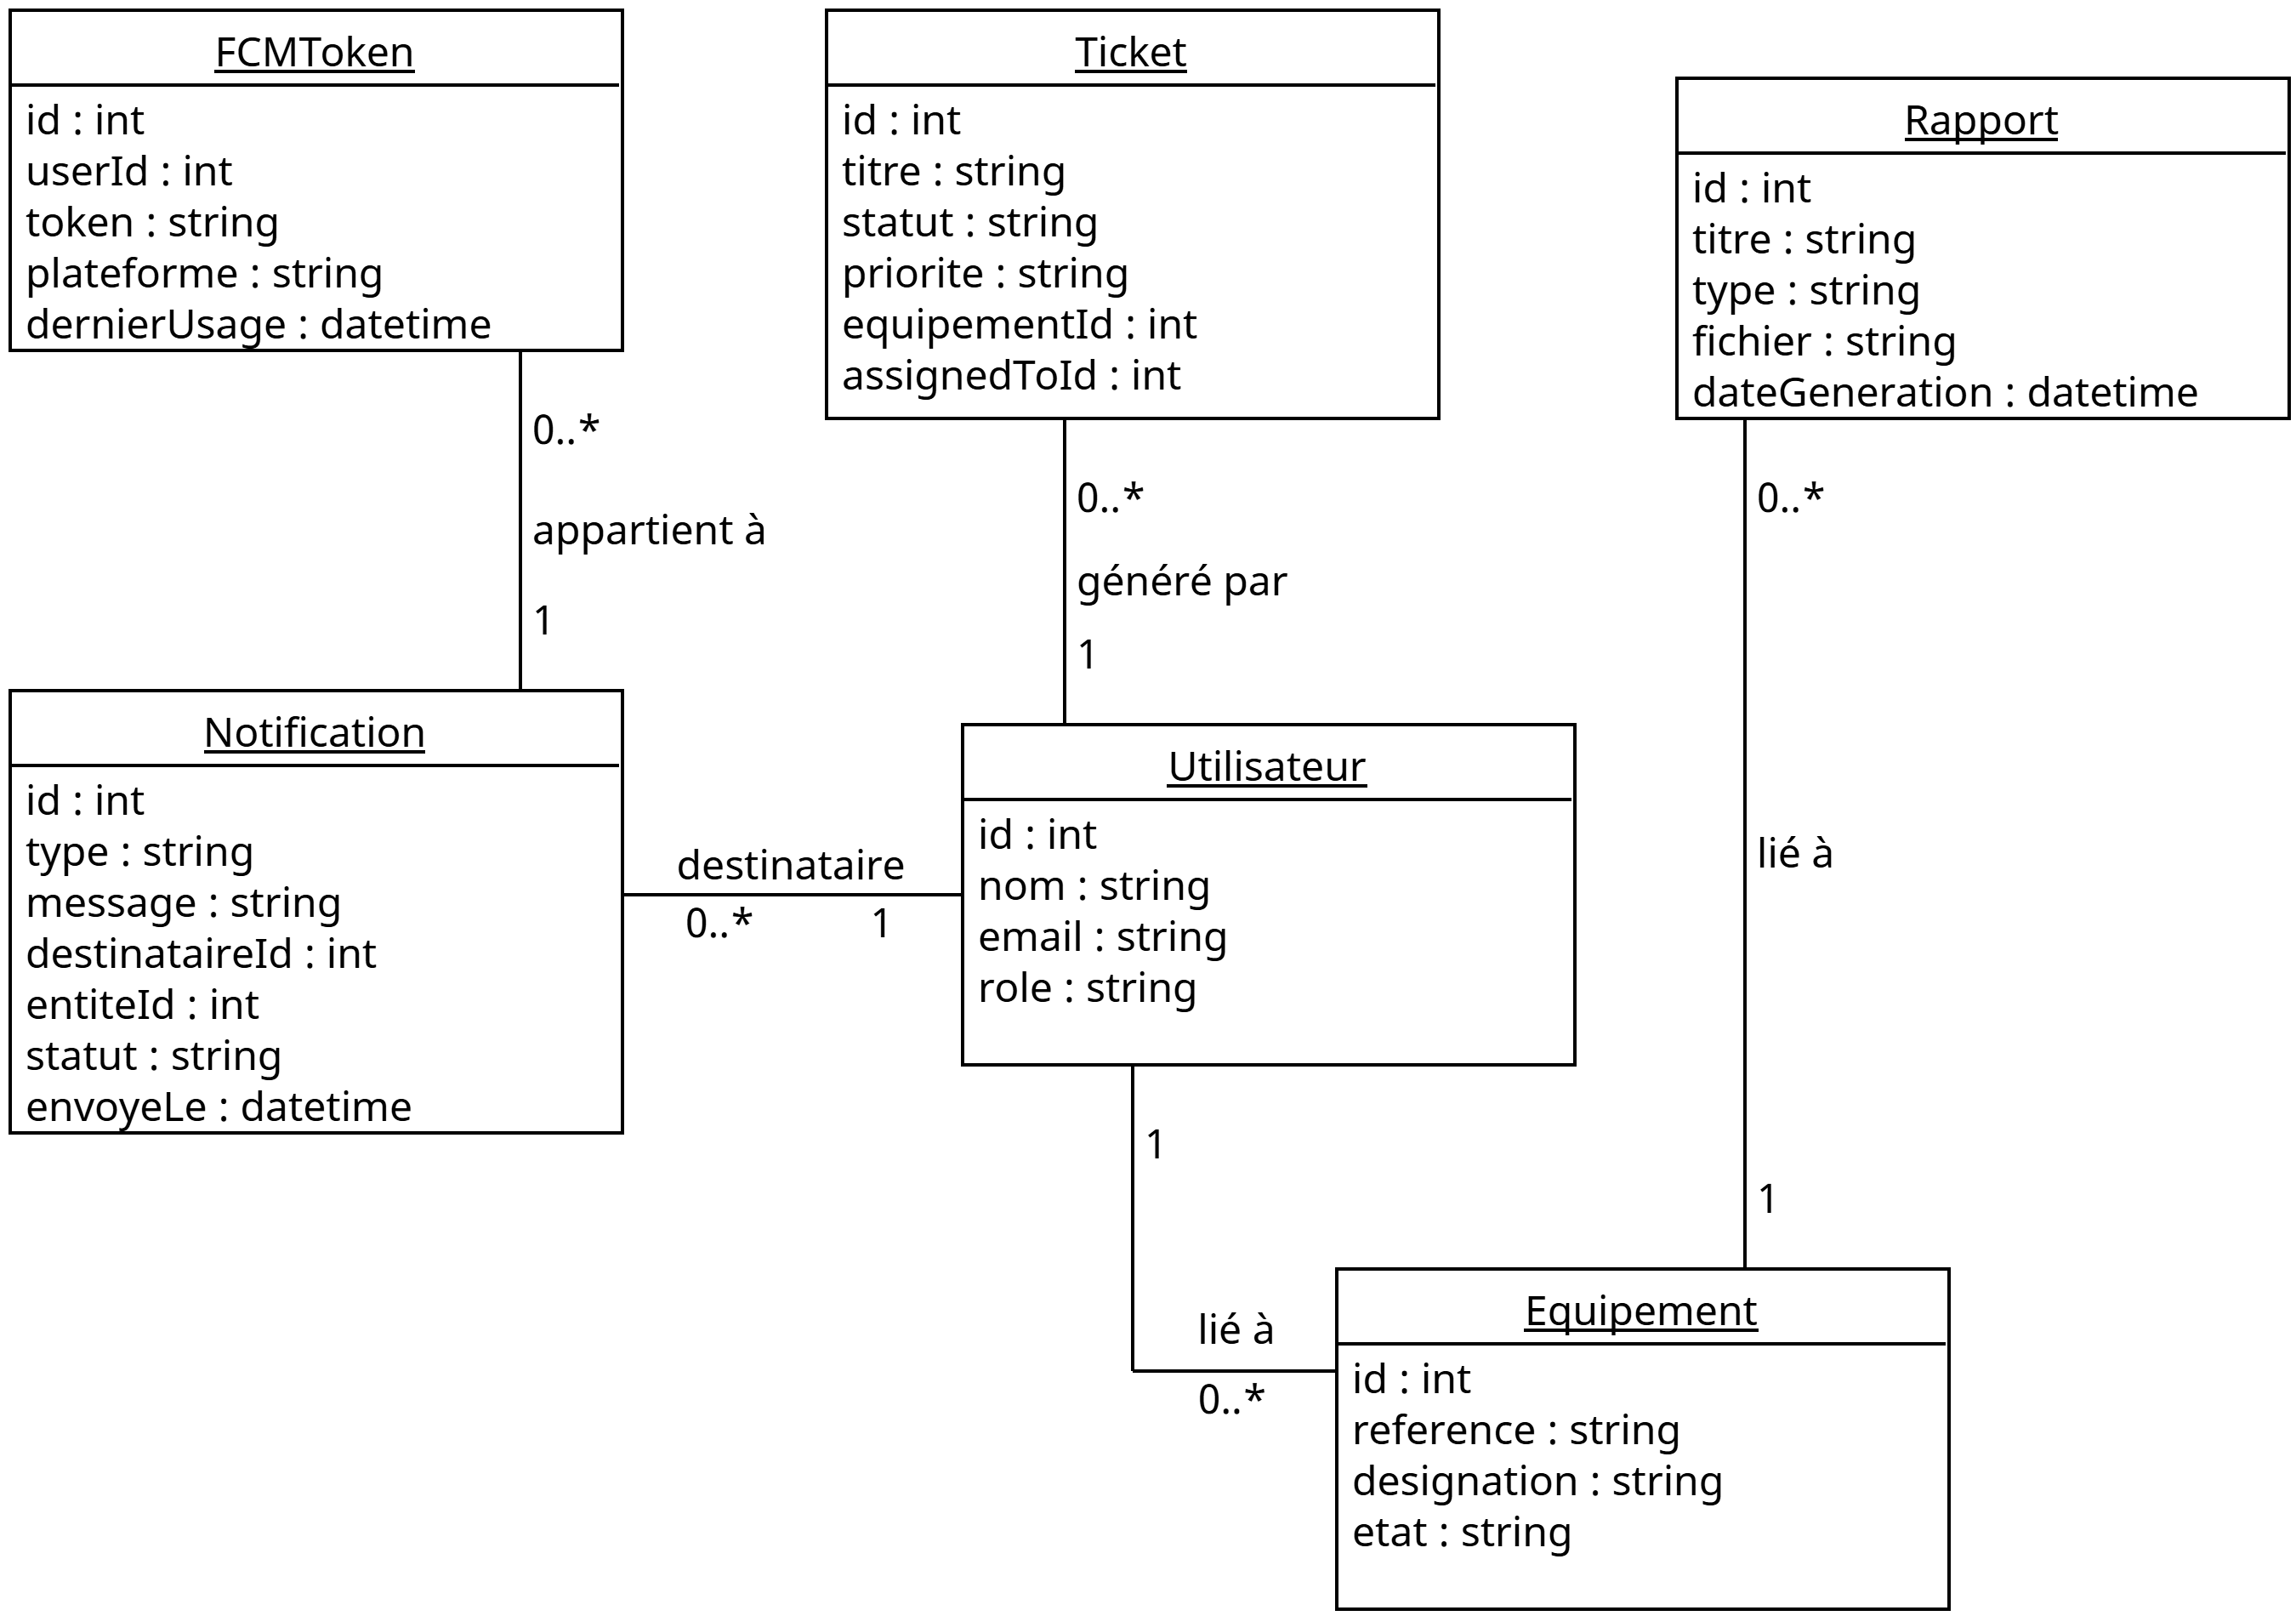
\includegraphics[width=0.9\textwidth]{chapter7/class_diagram_sprint3.png}
    \caption{Diagramme de classes du Sprint 3 — entités de notification et de reporting}
    \label{fig:class_diagram_sprint3}
\end{figure}

\subsection{Diagrammes de séquence du Sprint 3}

Les diagrammes de séquence ci-après décrivent les interactions dynamiques entre les acteurs et les composants du système lors de l'exécution des scénarios fonctionnels clés du Sprint 3. Ils constituent un outil de documentation de référence et un support de validation lors des revues de sprint.

% ---------------------------------------------------------
\subsubsection{Envoi d'une notification lors de la création d'un ticket}

Le processus débute lorsque l'utilisateur soumet le formulaire de déclaration d'incident depuis l'interface React. La requête \texttt{POST /api/tickets}, accompagnée du jeton JWT attestant l'authentification, est transmise au serveur Express. Celui-ci valide les données reçues, puis insère le ticket dans la base MySQL via Sequelize. Une fois la confirmation de persistance reçue, le backend diffuse une notification push à l'ensemble des utilisateurs disposant d'un jeton FCM enregistré, via la fonction \texttt{notifyAll()} du module \texttt{config/notifications.js}, qui délègue l'envoi FCM à \texttt{broadcastNotification()}. L'ensemble de ce traitement asynchrone est non bloquant pour la requête principale : la réponse \texttt{201 Created} est renvoyée au client React dès la confirmation de la persistance du ticket, indépendamment de la livraison effective des notifications.

\begin{figure}[H]
    \centering
    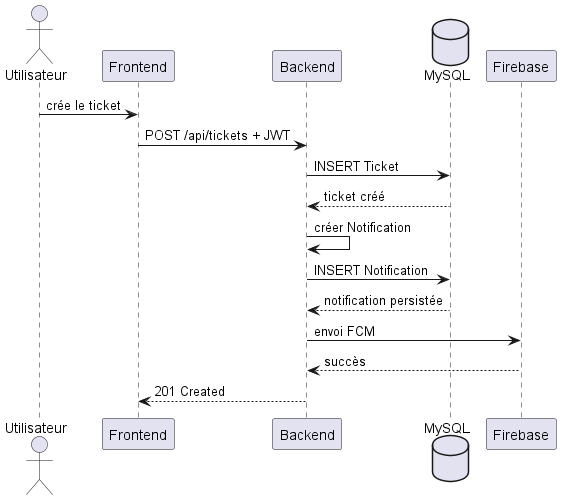
\includegraphics[width=0.9\textwidth]{chapter7/sequence_notification_creation_ticket.png}
    \caption{Diagramme de séquence — notification push lors de la création d'un ticket}
    \label{fig:sequence_notification_creation_ticket}
\end{figure}

% ---------------------------------------------------------
\subsubsection{Notification lors d'un changement de statut}

La Figure~\ref{fig:sequence_notification_statut} illustre le mécanisme de suivi déclenché lors de la mise à jour du statut d'un ticket par un technicien. Ce flux constitue un vecteur de communication essentiel entre les intervenants et les demandeurs, car il assure une traçabilité fonctionnelle sur l'avancement des incidents et prépare l'extension vers des notifications de suivi plus ciblées.

Lorsque le technicien modifie l'état d'un ticket — passage de \textit{ouvert} à \textit{assigne}, puis à \textit{en\_cours} et \textit{resolu} — la requête \texttt{PUT /api/tickets/\{id\}} est envoyée au backend. Après authentification du porteur de la requête et contrôle du rôle via \texttt{checkPermission}, Express valide la transition à l'aide de \texttt{utils/statusMachine.js}. Les transitions non autorisées sont rejetées avec une réponse \texttt{400 Bad Request}, ce qui évite les incohérences telles qu'une clôture prématurée. La version actuelle persiste la transition et les dates associées (\texttt{dateAssignation}, \texttt{dateResolution}, \texttt{dateCloture}) ; l'envoi ciblé d'une notification de suivi au demandeur constitue une évolution naturelle du même mécanisme \texttt{notifyAll()} / FCM.

\begin{figure}[H]
    \centering
    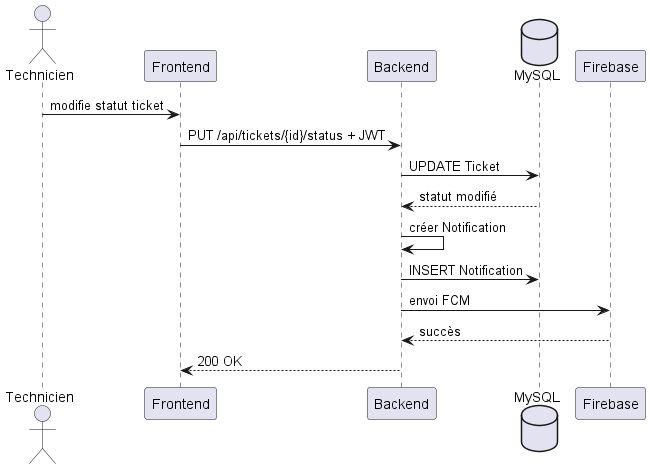
\includegraphics[width=0.9\textwidth]{chapter7/sequence_notification_statut.png}
    \caption{Diagramme de séquence — notification push lors d'un changement de statut de ticket}
    \label{fig:sequence_notification_statut}
\end{figure}

% ---------------------------------------------------------
\subsubsection{Consultation du tableau de bord}

La Figure~\ref{fig:sequence_consultation_dashboard} détaille le flux de données qui sous-tend l'affichage du tableau de bord analytique. Ce scénario illustre le parti pris architectural central du Sprint 3 : le calcul dynamique des KPI, plutôt que leur stockage redondant.

Lorsqu'un administrateur accède au tableau de bord, le frontend React émet une requête \texttt{GET /api/stats} authentifiée. Le backend Express intercepte cette requête puis calcule les indicateurs globaux par appels Sequelize \texttt{count()} sur les principales entités du système : équipements, tickets, interventions, maintenances, logiciels, licences, installations, rapports et utilisateurs. Il enrichit ces informations avec le taux de panne, l'âge moyen du parc et la répartition des tickets sur les six derniers mois. Le serveur consolide les résultats dans un objet JSON structuré et le retourne au frontend. React analyse cette réponse et injecte les données dans les composants graphiques (cartes KPI, histogrammes via Recharts), offrant à l'administrateur une vision synthétique et exploitable de l'état opérationnel du parc, mesurée dans le cadre de ce projet à une échelle locale.

\begin{figure}[H]
    \centering
    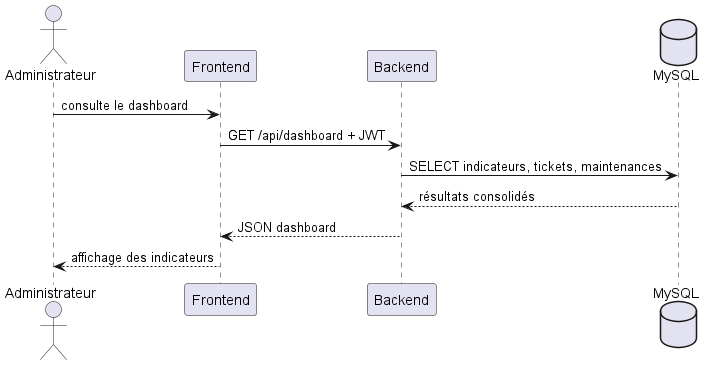
\includegraphics[width=0.9\textwidth]{chapter7/sequence_consultation_dashboard.png}
    \caption{Diagramme de séquence — consultation du tableau de bord analytique}
    \label{fig:sequence_consultation_dashboard}
\end{figure}

% ---------------------------------------------------------
\subsubsection{Génération d'un rapport}

La Figure~\ref{fig:sequence_generation_rapport} modélise le processus de génération à la demande d'un rapport d'activité. Ce flux est décisif pour les fonctions de contrôle de gestion et d'audit interne de l'établissement.

À l'initiative de l'administrateur, le frontend soumet une requête \texttt{POST /api/rapports} en précisant les paramètres du rapport souhaité (type de workflow, période, entités concernées). Le backend Express crée alors un enregistrement dans la table \texttt{Rapport}, ce qui assure la traçabilité de la demande. Pour la production documentaire, le frontend peut ensuite appeler \texttt{GET /api/rapports/\{id\}/pdf}, qui déclenche la génération à la volée d'un document PDF via PDFKit avec un en-tête professionnel FMM et les informations de l'équipement ou de l'opération concernée. Cette séparation entre création de l'enregistrement et génération du fichier évite de bloquer inutilement la requête de création et reste adaptée au prototype académique.

\begin{figure}[H]
    \centering
    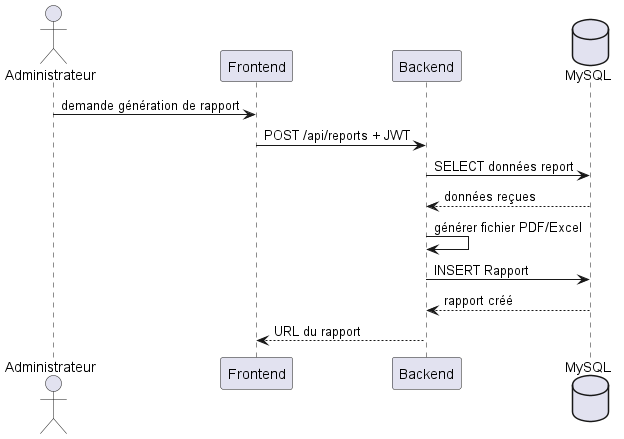
\includegraphics[width=0.9\textwidth]{chapter7/sequence_generation_rapport.png}
    \caption{Diagramme de séquence — génération d'un rapport d'activité PDF/Excel}
    \label{fig:sequence_generation_rapport}
\end{figure}

% ---------------------------------------------------------
\subsubsection{Export des statistiques}

La Figure~\ref{fig:sequence_export_statistics} présente le mécanisme d'export des statistiques brutes du système. Ce flux se distingue de la génération de rapports par sa vocation plus analytique : il s'agit ici de fournir les données agrégées dans un format exploitable par des outils tiers (tableurs, outils de Business Intelligence).

À la réception de la requête \texttt{GET /api/rapports/export/excel}, le backend extrait directement l'inventaire depuis la table \texttt{Equipement} et met en forme les colonnes essentielles : identifiant, numéro d'inventaire, numéro de série, marque, modèle, catégorie, date d'achat et statut courant. Le fichier est généré avec ExcelJS et transmis au client comme pièce jointe grâce à l'en-tête HTTP \texttt{Content-Disposition}. De manière complémentaire, un endpoint PDF dédié permet d'exporter les rapports via PDFKit. Cette approche permet de disposer de données actualisées à la demande, sans surcharge de la base de données par des tables de cache redondantes.

\begin{figure}[H]
    \centering
    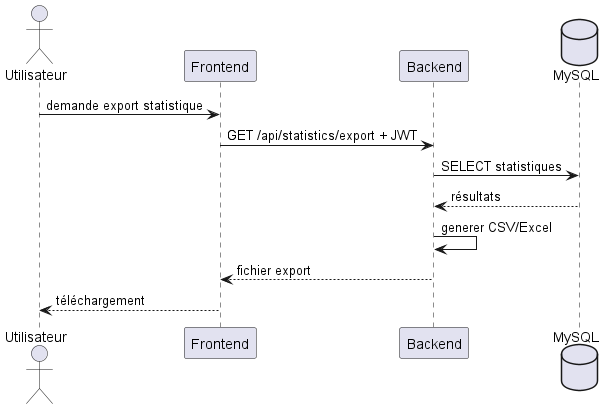
\includegraphics[width=0.9\textwidth]{chapter7/sequence_export_statistics.png}
    \caption{Diagramme de séquence — export des statistiques du parc informatique}
    \label{fig:sequence_export_statistics}
\end{figure}

% =========================================================
\section{Tableaux de bord et interfaces utilisateur}
\label{sec:dashboards}

L'interface web développée au cours du Sprint 3 constitue la vitrine opérationnelle de l'ensemble du système. Elle traduit, sous une forme visuelle intuitive et interactive, la richesse du modèle de données construit lors des itérations précédentes. La conception de cette couche de présentation a été guidée par trois principes fondamentaux : la \textbf{personnalisation par rôle} (chaque profil accède à une vue adaptée à ses responsabilités), la \textbf{lisibilité immédiate} (les indicateurs critiques sont mis en avant visuellement, sans nécessiter d'interprétation préalable) et la \textbf{réactivité} (les données sont chargées de manière asynchrone pour ne pas pénaliser la navigation).

\textbf{Note architecturale :} L'interface de tableau de bord est implémentée comme un \textbf{composant unique adaptatif} (\texttt{Dashboard.jsx}), dont le contenu est conditionné dynamiquement en fonction du rôle de l'utilisateur authentifié (via la propriété \texttt{user.role} du contexte d'authentification). Cette approche à composant polymorphe favorise la maintenabilité : toute évolution du tableau de bord peut s'appliquer uniformément à tous les profils depuis un point d'entrée unique.

% ---------------------------------------------------------
\subsection{Tableau de bord administrateur}

Le tableau de bord administrateur, illustré par la Figure~\ref{fig:admin_dash}, est l'interface de pilotage la plus fonctionnelle du système. Conçu pour l'administrateur du SmartLab, il agrège l'ensemble des indicateurs stratégiques du parc informatique sur un écran unique, permettant une prise de décision rapide et éclairée.

La partie supérieure de l'interface présente quatre cartes KPI synthétiques : le nombre total d'équipements recensés dans l'inventaire, le nombre de tickets d'incident actuellement ouverts, le nombre d'interventions planifiées pour la semaine en cours, et le taux global de disponibilité du parc. Ces métriques sont calculées à chaque chargement de la page par des requêtes SQL d'agrégation exécutées côté serveur, ce qui permet d'afficher des indicateurs actualisés dans le périmètre du prototype.

La section centrale offre une représentation graphique de la distribution des équipements par statut opérationnel (fonctionnel, en panne, en maintenance, réformé) et par catégorie matérielle. Ces visualisations, réalisées avec la bibliothèque \textbf{Recharts} intégrée à l'écosystème React, permettent à l'administrateur d'identifier immédiatement les catégories les plus touchées par des pannes ou les périodes de forte demande d'intervention.

La partie inférieure présente la liste des derniers tickets déclarés, avec leur statut, leur priorité et le technicien affecté, ainsi qu'un calendrier des maintenances préventives à venir. L'administrateur peut depuis cette interface naviguer vers le détail de n'importe quelle entité en un seul clic, rendant le tableau de bord à la fois un outil de supervision globale et un point d'entrée vers la gestion opérationnelle fine.

\begin{figure}[H]
    \centering
    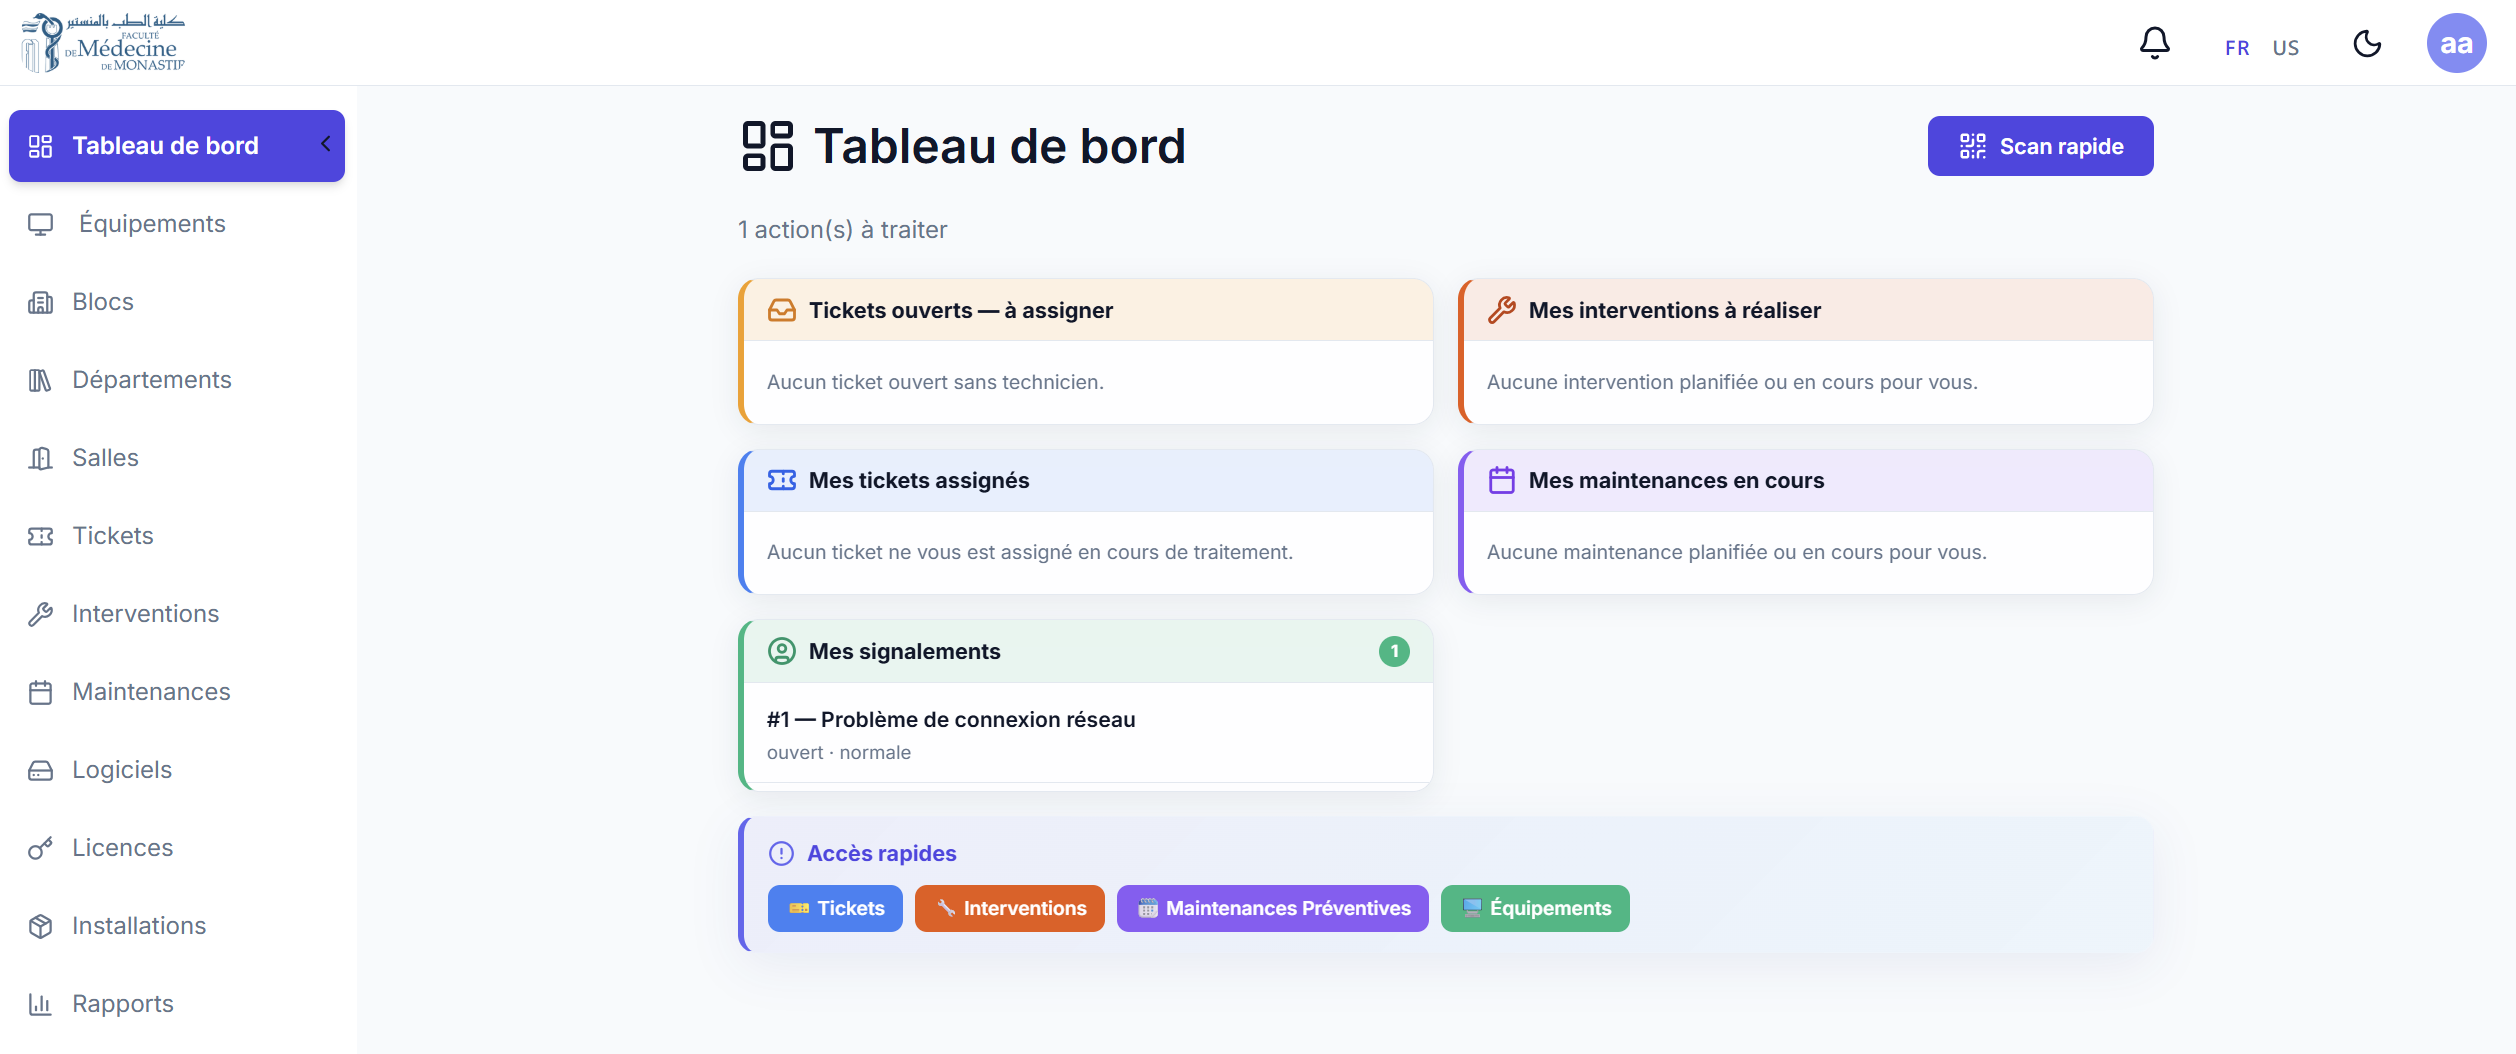
\includegraphics[width=1\textwidth]{chapter7/screens/AdminDash.png}
    \caption{Tableau de bord administrateur — vue globale des KPI et de l'état opérationnel du parc}
    \label{fig:admin_dash}
\end{figure}

% ---------------------------------------------------------
\subsection{Tableau de bord utilisateur}

La Figure~\ref{fig:user_dash} présente l'interface destinée aux utilisateurs finaux du parc informatique — typiquement, les enseignants-chercheurs, personnels administratifs et étudiants en thèse utilisant les ressources informatiques du SmartLab. La conception de cette interface obéit à un principe d'épuration maximale : seules les informations directement utiles à cet acteur sont affichées, à l'exclusion de toute donnée d'administration ou de configuration qui relève de responsabilités distinctes.

L'écran principal présente à l'utilisateur la liste des tickets qu'il a déclarés, avec leur statut courant et la date de dernière mise à jour. Ce suivi transparent de l'avancement des demandes réduit le besoin de relances auprès du service technique et renforce la confiance de l'utilisateur dans la fiabilité du processus de maintenance. Un journal des notifications reçues (alertes de prise en charge, confirmation de résolution) enrichit cette vue.

\begin{figure}[H]
    \centering
    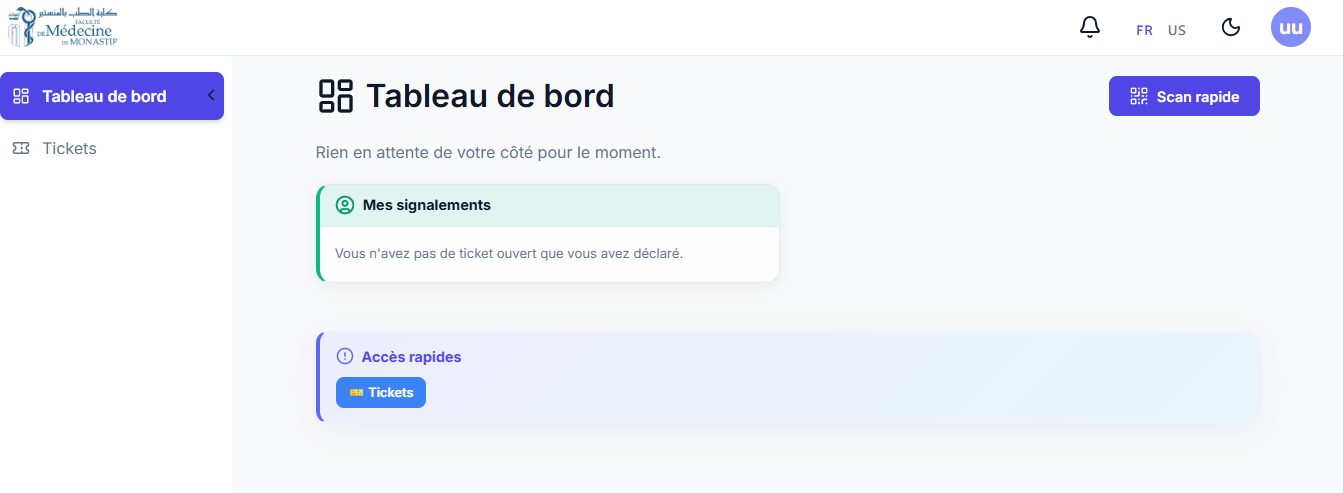
\includegraphics[width=1\textwidth]{chapter7/screens/UserDash.png}
    \caption{Tableau de bord utilisateur — suivi des équipements affectés et des demandes d'intervention}
    \label{fig:user_dash}
\end{figure}

% ---------------------------------------------------------
\subsection{Tableau de bord technicien}

La Figure~\ref{fig:tech_dash} illustre l'interface de travail quotidien du technicien de maintenance. Contrairement aux tableaux de bord précédents qui s'inscrivent dans une logique de supervision et de suivi, celui-ci est résolument orienté vers l'action et l'efficacité opérationnelle sur le terrain.

La vue principale liste l'ensemble des tickets affectés au technicien connecté, triés par ordre de priorité décroissante. Chaque ticket est présenté avec les informations essentielles à son traitement : désignation et localisation physique de l'équipement concerné (bloc, département, salle), description de la panne signalée par l'utilisateur, date de création et délai cible de résolution. Un code couleur intuitif — rouge pour les tickets critiques, orange pour les priorités hautes, vert pour les interventions planifiées — permet au technicien de hiérarchiser immédiatement son plan de travail de la journée.

Le technicien peut directement modifier le statut d'un ticket depuis cette interface (passage à \textit{en cours} lors de la prise en charge, puis à \textit{résolu} à l'issue de l'intervention), ce qui déclenche automatiquement la notification push vers l'utilisateur demandeur. Une section dédiée recense les maintenances préventives planifiées pour la semaine, permettant une organisation proactive du travail et évitant les conflits d'agenda entre interventions correctives et préventives.

\begin{figure}[H]
    \centering
    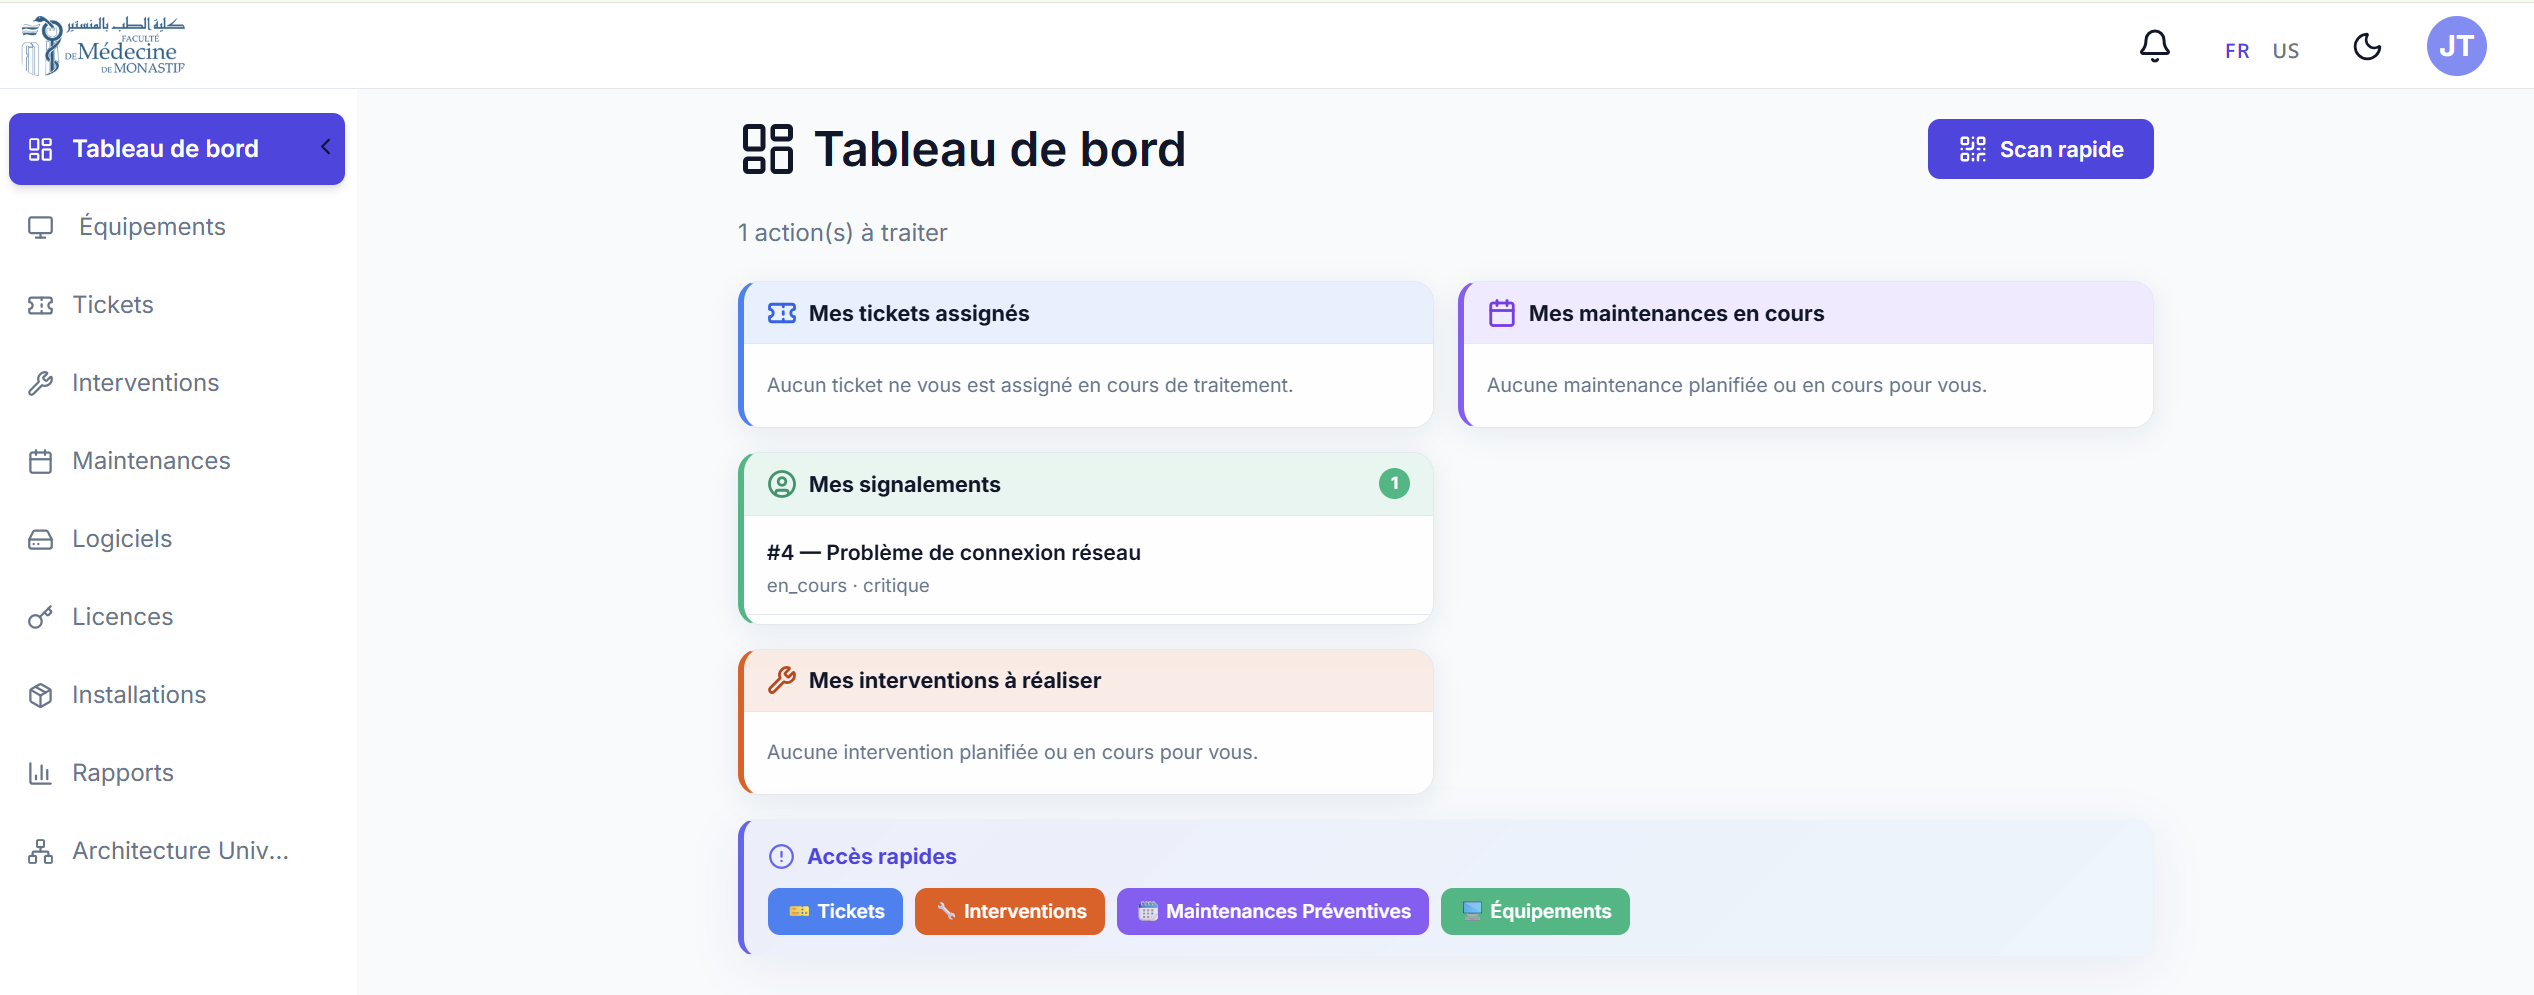
\includegraphics[width=1\textwidth]{chapter7/screens/TechDash.png}
    \caption{Tableau de bord technicien — file d'attente des interventions classées par priorité}
    \label{fig:tech_dash}
\end{figure}

% =========================================================
\section{Modules de gestion du parc informatique}
\label{sec:modules_gestion}

Au-delà des tableaux de bord de supervision, le Sprint 3 consolide et enrichit les modules de gestion opérationnelle introduits lors des sprints précédents. Ces modules constituent le cœur du système et permettent de gérer le cycle de vie des actifs informatiques de la FMM.

% ---------------------------------------------------------
\subsection{Gestion de l'inventaire et des équipements}

\subsubsection{Inventaire des équipements}

La Figure~\ref{fig:admin_equipment} présente l'interface centrale de gestion de l'inventaire informatique. Cette vue est accessible exclusivement à l'administrateur du système et constitue le référentiel principal de l'ensemble du parc matériel de la FMM.

L'interface adopte une présentation tabulaire enrichie qui liste les équipements enregistrés dans la base de données, avec leurs attributs essentiels : référence constructeur, désignation, catégorie matérielle, état opérationnel, localisation physique (bloc et salle), et utilisateur affecté. Un système de filtres multicritères dynamiques permet de restreindre l'affichage selon plusieurs combinaisons de ces attributs — par exemple, afficher uniquement les ordinateurs portables du Département de Biologie Médicale dont le statut est \textit{en panne}. Cette capacité de filtrage précise est particulièrement précieuse lors des inventaires physiques périodiques ou lors de la préparation de rapports sectoriels.

Depuis chaque ligne du tableau, l'administrateur dispose d'un menu d'actions contextuelles permettant de consulter la fiche détaillée de l'équipement, d'initier un transfert vers une autre localisation, de modifier ses attributs ou de le retirer de l'inventaire actif. La liste intègre également une pagination intelligente qui maintient la fluidité de l'interface même pour des inventaires de plusieurs centaines d'équipements.

\begin{figure}[H]
    \centering
    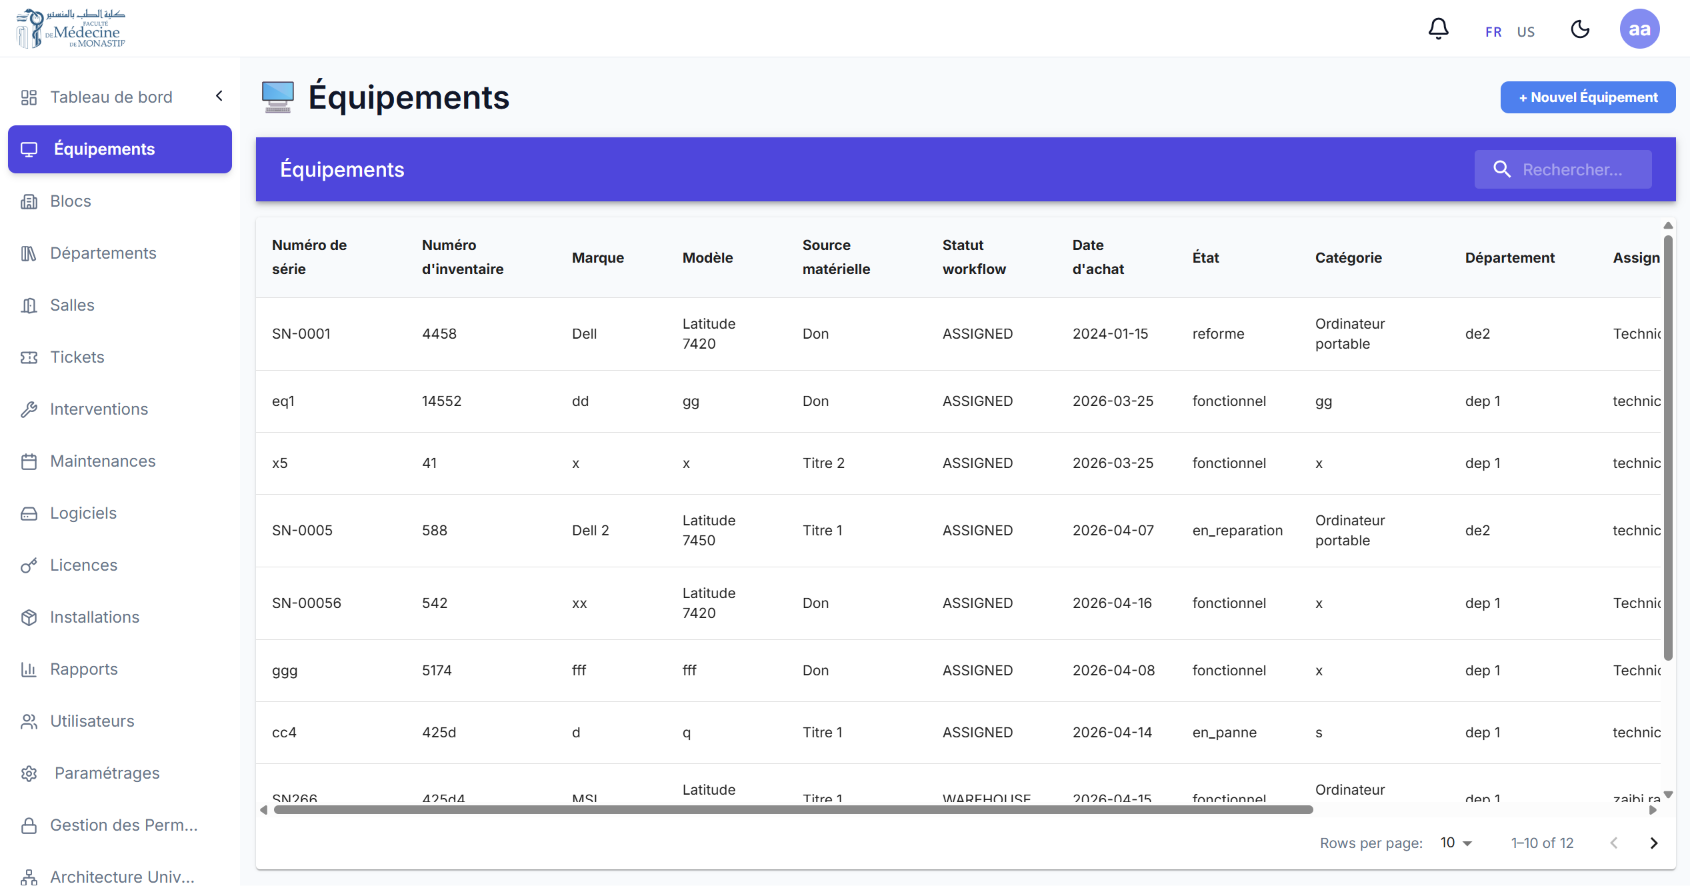
\includegraphics[width=1\textwidth]{chapter7/screens/AdminEquipment.png}
    \caption{Interface de gestion de l'inventaire — liste filtrée des équipements du parc}
    \label{fig:admin_equipment}
\end{figure}

\subsubsection{Enregistrement d'un nouvel équipement}

La Figure~\ref{fig:new_equipment} présente le formulaire d'enregistrement d'un nouvel actif informatique dans le système. Ce formulaire est le point d'entrée de tout équipement dans le cycle de vie géré par la plateforme, et sa conception reflète le souci de rigueur et de cohérence qui caractérise l'ensemble du système.

Le formulaire est structuré en sections thématiques pour faciliter la saisie et réduire les risques d'erreur : identification de l'équipement (référence, désignation, numéro de série, marque, modèle), caractéristiques techniques (catégorie, date d'acquisition, valeur d'achat, état initial), affectation organisationnelle (bloc, département, salle, utilisateur responsable) et configuration logicielle (systèmes d'exploitation et logiciels associés, gérés par liaison avec les entités \texttt{Logiciel} et \texttt{Licence}).

Chaque champ est soumis à des validations côté client et côté serveur : l'unicité du numéro de série est vérifiée en base de données avant l'insertion, la cohérence de la localisation (la salle doit appartenir au département, lui-même rattaché au bloc sélectionné) est contrôlée par le backend. À la validation du formulaire, le backend Express persiste l'entité \texttt{Equipement} et déclenche immédiatement la génération du QR code associé, encodant l'identifiant UUID unique de l'équipement. Ce QR code est stocké en base et rendu disponible pour impression et apposition physique sur la machine, dans une version implémentée de manière simplifiée afin de rester adaptée au contexte académique.

\begin{figure}[H]
    \centering
    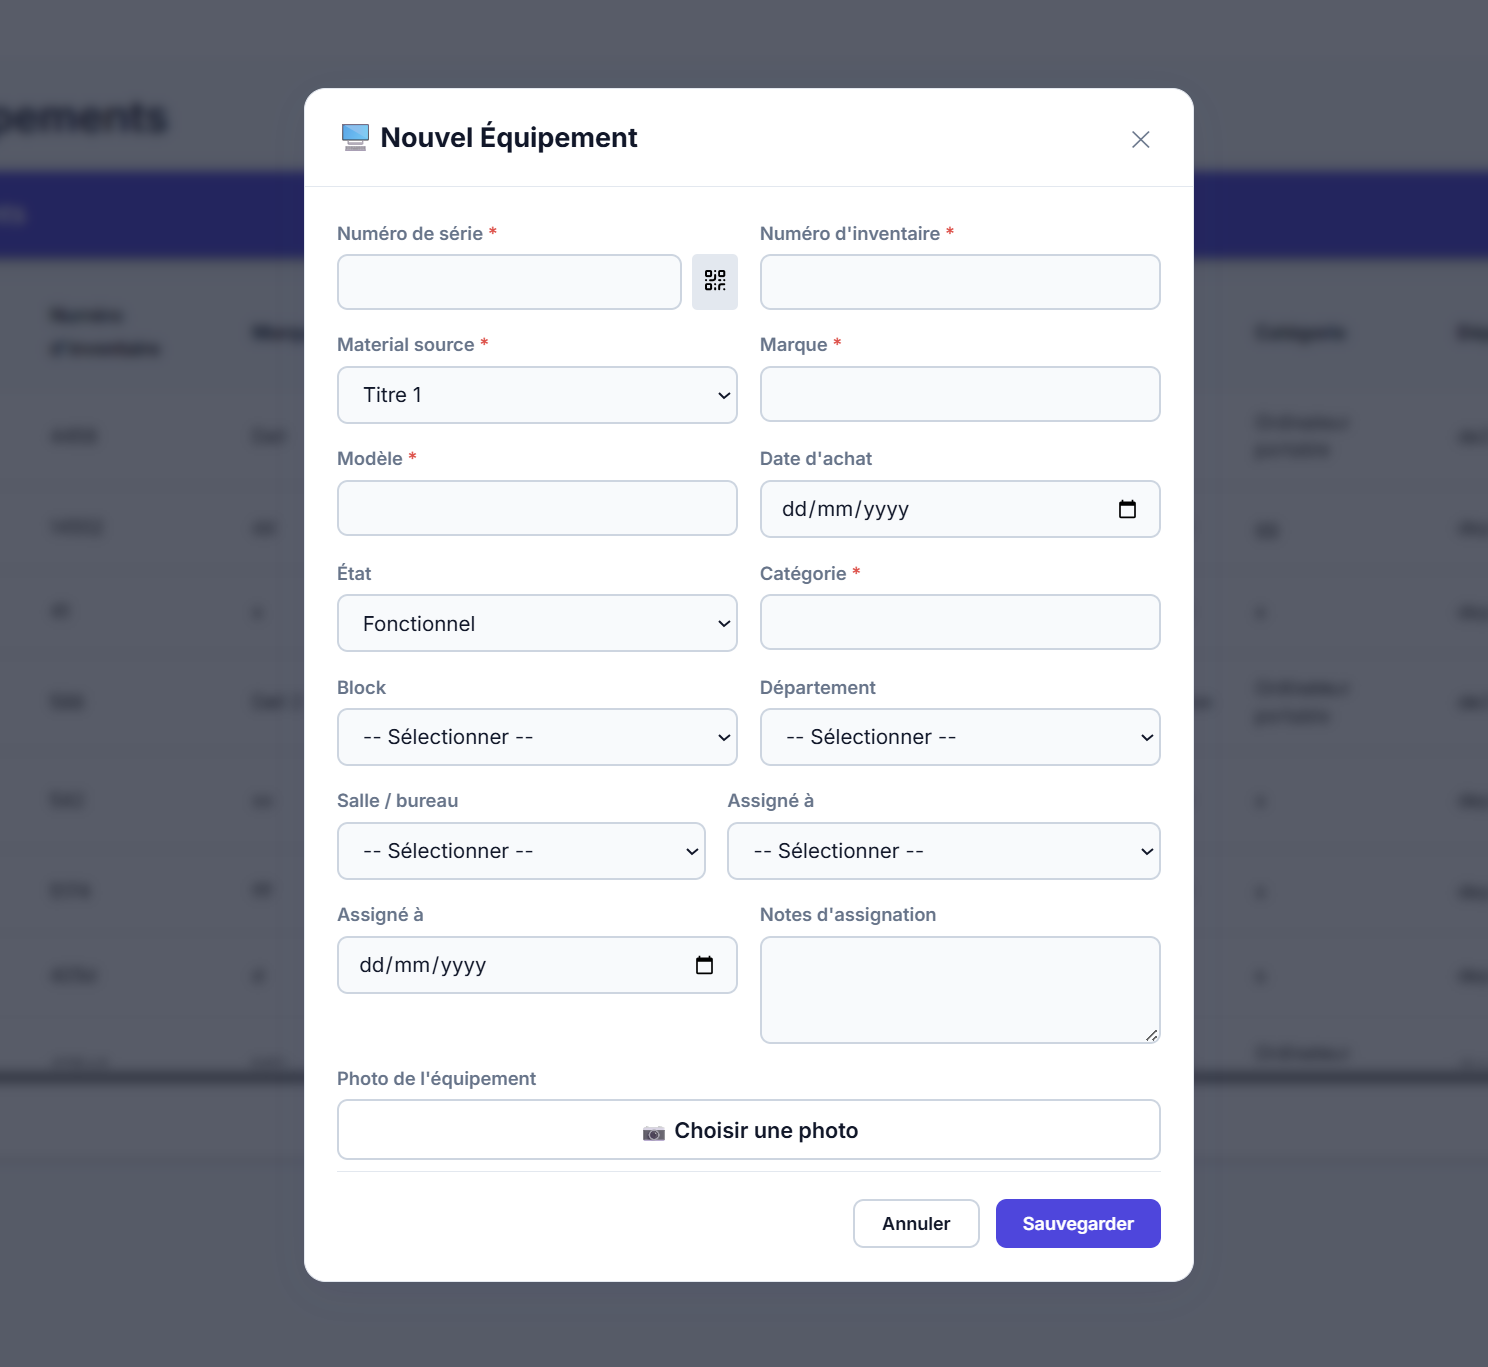
\includegraphics[width=1\textwidth]{chapter7/screens/NewEquiment.png}
    \caption{Formulaire d'enregistrement d'un nouvel équipement avec génération automatique du QR code}
    \label{fig:new_equipment}
\end{figure}

% ---------------------------------------------------------
\subsection{Contrôle d'accès par rôles (RBAC)}

La Figure~\ref{fig:permission_management} illustre le module de gestion des permissions. Des mécanismes de sécurité de base ont été implémentés, notamment l’authentification JWT et le contrôle d’accès basé sur les rôles (RBAC). Cette dimension sécuritaire est importante dans un environnement institutionnel comme la FMM, où des données liées aux actifs matériels et aux identités des personnels sont traitées quotidiennement.

Le système définit trois rôles primaires — \textit{Administrateur}, \textit{Technicien} et \textit{Utilisateur} — auxquels sont associées des matrices de permissions granulaires définissant les opérations autorisées sur chaque ressource de l'API (\texttt{GET}, \texttt{POST}, \texttt{PUT}, \texttt{DELETE} sur les endpoints \texttt{/api/equipements}, \texttt{/api/tickets}, \texttt{/api/users}, etc.). L'interface présentée dans la Figure~\ref{fig:permission_management} permet à l'administrateur de visualiser et de modifier cette matrice de permissions, d'affecter des rôles aux utilisateurs et, si nécessaire, de créer des profils personnalisés combinant des sous-ensembles de permissions pour des cas d'usage spécifiques.

Le contrôle des accès est appliqué systématiquement par un middleware Express placé en amont de chaque route protégée. Ce middleware décode le jeton JWT présenté dans l'en-tête de la requête, extrait le rôle de l'utilisateur authentifié et vérifie sa conformité avec les permissions requises. En cas de violation, une réponse \texttt{403 Forbidden} est renvoyée immédiatement, sans que la logique métier sous-jacente soit exécutée.

\begin{figure}[H]
    \centering
    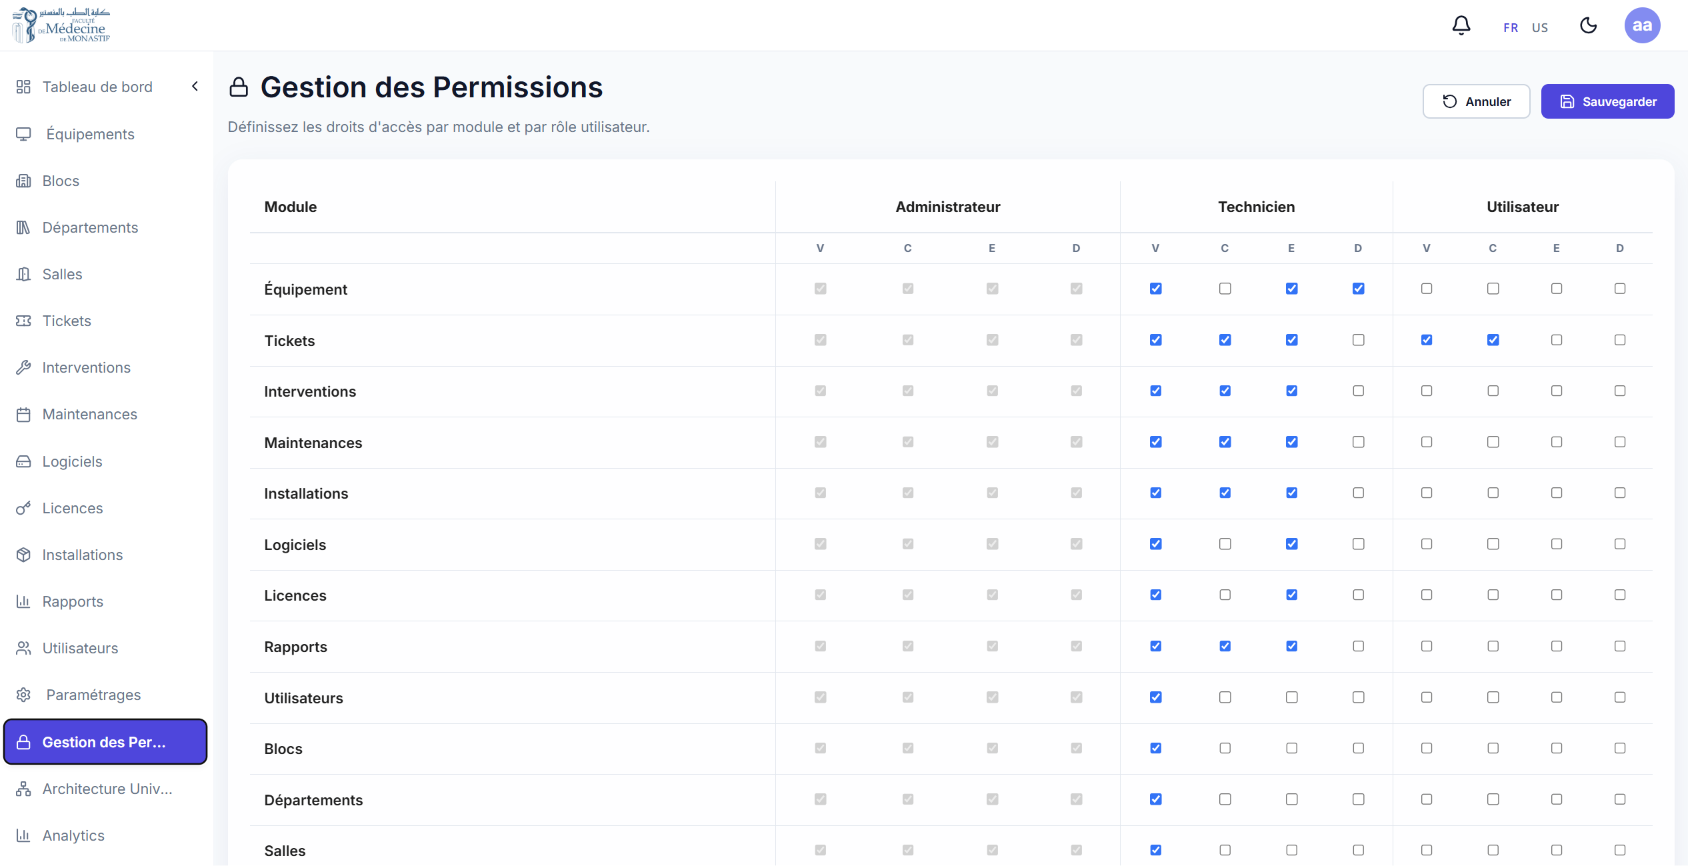
\includegraphics[width=1\textwidth]{chapter7/screens/Permission.png}
    \caption{Interface de gestion des permissions et rôles — modèle RBAC du système}
    \label{fig:permission_management}
\end{figure}

% ---------------------------------------------------------
\subsection{Analyse et reporting}

\subsubsection{Module analytique du parc}

La Figure~\ref{fig:analytics} présente le module d'analyse décisionnelle du parc informatique. Cette interface se distingue du tableau de bord opérationnel par sa vocation prospective : là où le tableau de bord offre une photographie instantanée de l'état du système, le module analytique propose une lecture des tendances historiques et des patterns d'utilisation sur des périodes configurables.

Les visualisations disponibles couvrent plusieurs dimensions analytiques complémentaires. L'évolution mensuelle du volume de tickets sur les douze derniers mois permet d'identifier les périodes de forte sinistralité et d'anticiper les besoins en ressources humaines techniques. La distribution des pannes par catégorie d'équipement révèle les typologies matérielles les plus fragiles ou les plus sollicitées, orientant ainsi les décisions d'investissement et de renouvellement du parc. Le taux de résolution par technicien, exprimé en délai moyen de clôture (MTTR — \textit{Mean Time To Repair}), fournit une mesure objective de la performance individuelle des équipes techniques.

Ces analyses sont produites par des requêtes SQL d'agrégation exécutées dynamiquement par le backend, sans recours à une couche de cache ou à une table de faits dédiée. Ce choix permet de présenter des résultats proches de l'état courant de la base de données, sans décalage temporel volontaire.

\begin{figure}[H]
    \centering
    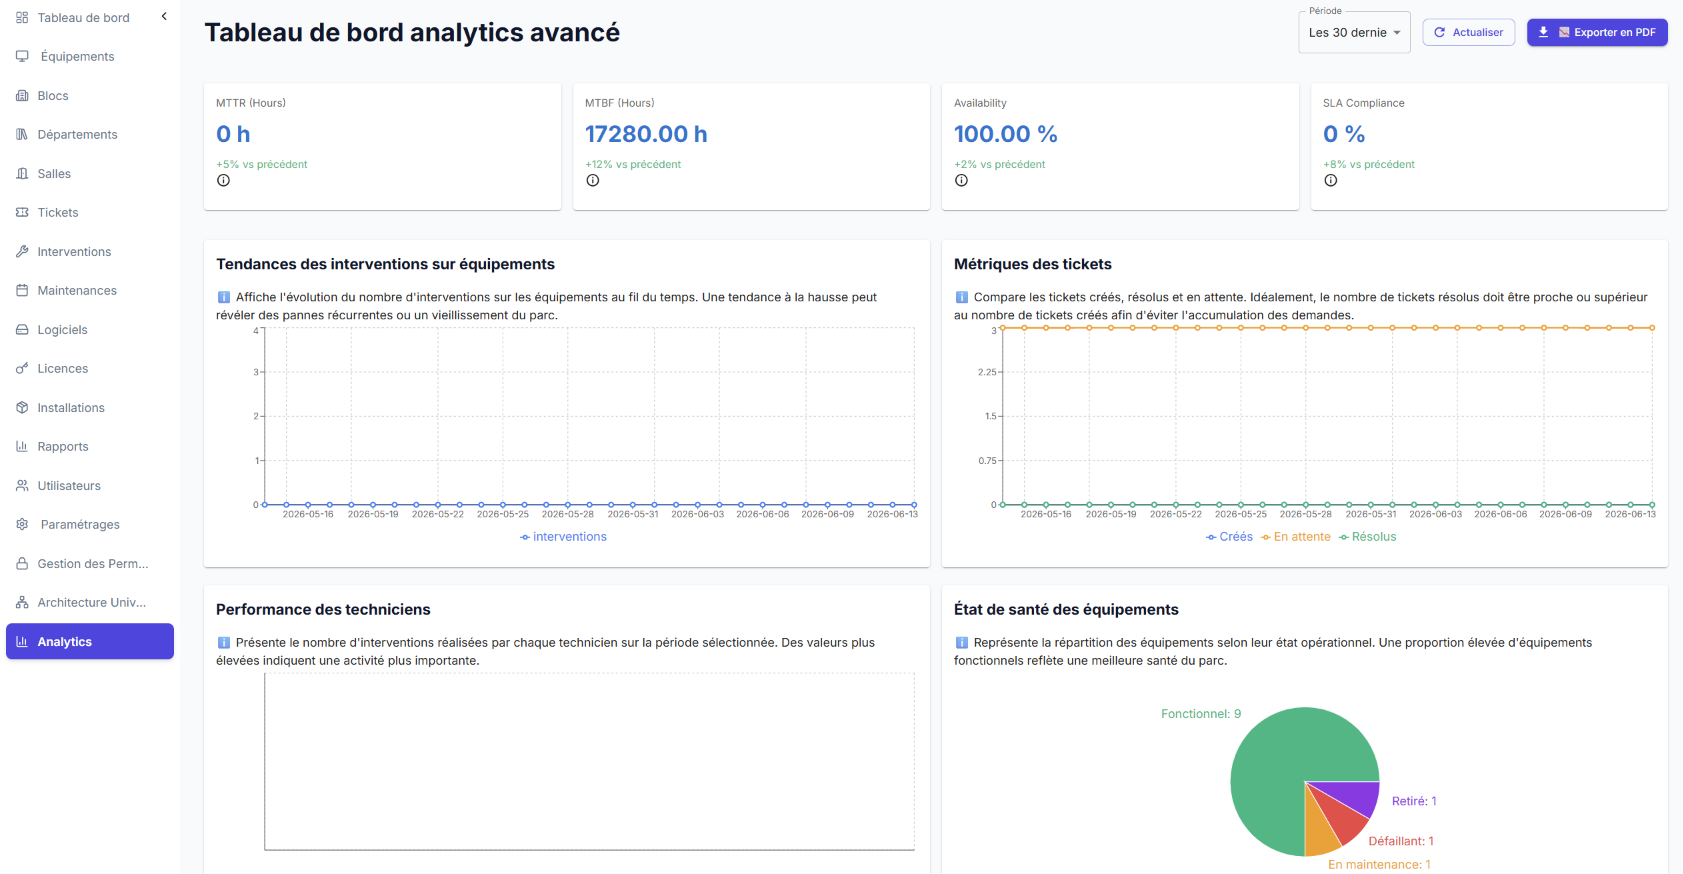
\includegraphics[width=1\textwidth]{chapter7/screens/Analytics.png}
    \caption{Module analytique — tendances de pannes et indicateurs de performance du parc}
    \label{fig:analytics}
\end{figure}

\subsubsection{Génération et consultation des rapports}

La Figure~\ref{fig:reports} illustre le module de génération de rapports de workflow et d'inventaire. Ce module répond à une exigence institutionnelle forte~: assurer la traçabilité formelle des opérations sur les actifs informatiques de la FMM.

Le module gère deux catégories de documents. La première couvre les \textbf{rapports de workflow} : à chaque opération de décharge (affectation d'équipement), de transfert ou de mise en réforme, le système génère automatiquement un document PDF structuré, avec en-tête FMM professionnel (logo, date, opérateur), fiche descriptive de l'équipement et résumé de l'opération. Un enregistrement correspondant est créé dans la table \texttt{Rapport}, assurant la traçabilité fonctionnelle de chaque mouvement d'actif. La deuxième catégorie couvre l'\textbf{export inventaire} : un export Excel du parc est disponible via \texttt{GET /api/rapports/export/excel}, généré avec la bibliothèque ExcelJS. Ce document consolide l'ensemble des actifs avec leurs attributs, leur localisation et leur état, facilitant les audits physiques ponctuels.

\begin{figure}[H]
    \centering
    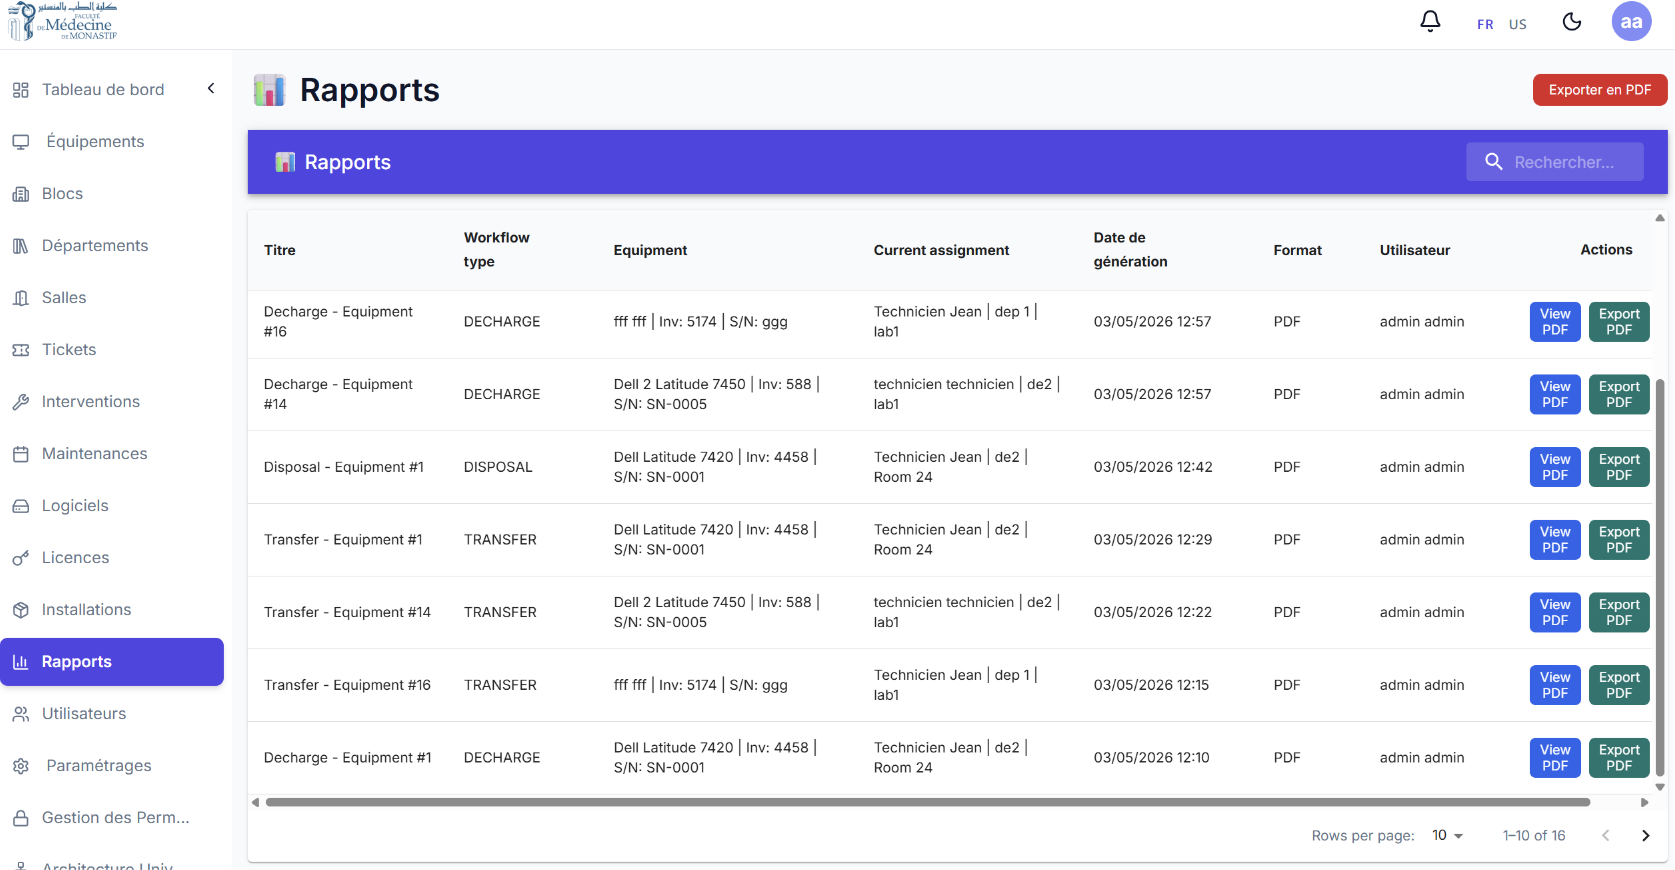
\includegraphics[width=1\textwidth]{chapter7/screens/Rapports.png}
    \caption{Module de reporting — génération de rapports périodiques PDF/Excel et consultation des archives}
    \label{fig:reports}
\end{figure}

% ---------------------------------------------------------
\subsection{Architecture physique et traçabilité des actifs}

\subsubsection{Visualisation de l'architecture physique}

La Figure~\ref{fig:architecture} représente la vue d'architecture physique du parc informatique, qui matérialise dans l'interface la hiérarchie organisationnelle réelle de la FMM : \textbf{Bloc} $\rightarrow$ \textbf{Département} $\rightarrow$ \textbf{Salle} $\rightarrow$ \textbf{Équipement}. Cette représentation arborescente est l'une des fonctionnalités les plus distinctives du système, car elle permet de contextualiser chaque actif informatique dans son environnement physique réel, bien au-delà d'un simple inventaire tabulaire.

L'administrateur peut naviguer dans cet arbre en développant successivement les nœuds de la hiérarchie, jusqu'à accéder à la liste des équipements présents dans une salle donnée. Depuis chaque nœud, des métriques agrégées sont affichées : nombre total d'équipements dans le bloc ou le département, nombre d'équipements opérationnels vs. en panne, nombre de tickets ouverts associés à cette zone. Cette visualisation facilite grandement les audits physiques en permettant de préparer une tournée d'inspection de manière structurée, salle par salle.

\begin{figure}[H]
    \centering
    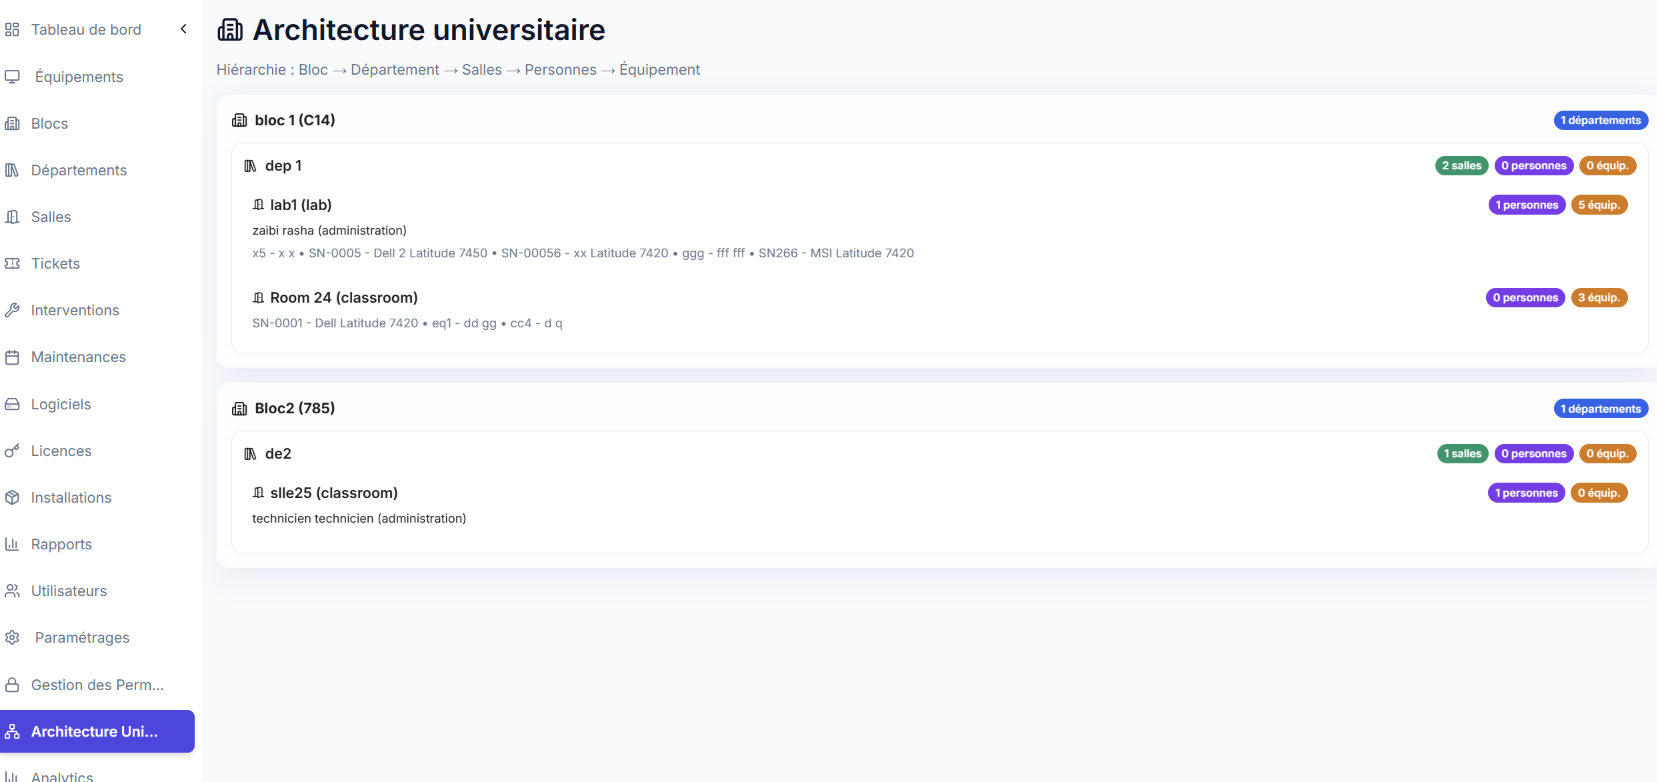
\includegraphics[width=1\textwidth]{chapter7/screens/Architecture.png}
    \caption{Vue d'architecture physique — hiérarchie Bloc/Département/Salle/Équipement de la FMM}
    \label{fig:architecture}
\end{figure}

\subsubsection{Génération et affichage du QR code d'un équipement}

La Figure~\ref{fig:view_qr} présente l'interface d'affichage du QR code associé à un équipement spécifique. Chaque actif informatique enregistré dans le système se voit attribuer un identifiant UUID unique, encodé dans un QR code généré par le backend au moment de l'enregistrement de l'équipement. Ce code à deux dimensions constitue le pivot du mécanisme d'identification physique rapide, qui représente une fonctionnalité utile de la plateforme dans le contexte institutionnel tunisien.

L'interface présente le QR code dans une résolution optimale pour l'impression, accompagné des informations d'identification essentielles de l'équipement (référence, désignation, localisation). Un bouton d'impression directe permet de générer une étiquette formatée à apposer sur la machine physique. Une fois cette étiquette collée sur l'équipement, il devient possible d'interagir instantanément avec sa fiche système sans aucune saisie manuelle, simplement en le scannant avec un terminal mobile.

\begin{figure}[H]
    \centering
    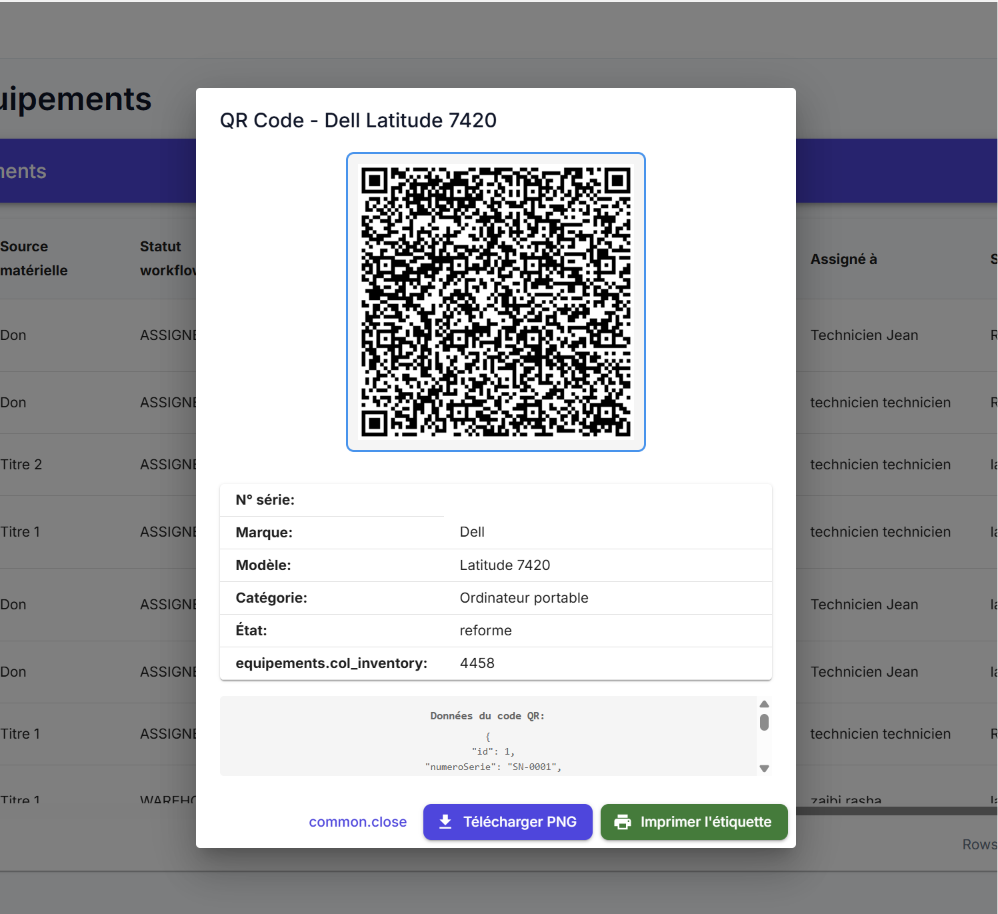
\includegraphics[width=1\textwidth]{chapter7/screens/ViewQR.png}
    \caption{Interface d'affichage et d'impression du QR code d'un équipement}
    \label{fig:view_qr}
\end{figure}

\subsubsection{Scan du QR code sur le terrain}

La Figure~\ref{fig:scan_qr} illustre l'interface de scan du QR code, conçue pour un usage mobile sur le terrain. Lorsqu'un technicien est appelé à intervenir sur une machine ou qu'un administrateur réalise un audit physique, il lui suffit de pointer la caméra de son terminal mobile vers l'étiquette QR code apposée sur l'équipement. L'application web, optimisée pour les navigateurs mobiles, active la caméra et décode le QR en temps réel.

Le décodage du QR code extrait l'UUID de l'équipement et déclenche une navigation automatique vers la fiche détaillée correspondante dans le système. En quelques secondes, le technicien dispose de l'ensemble des informations relatives à la machine : historique fonctionnel des interventions passées, état actuel (opérationnel, en panne, en maintenance), tickets en cours associés, spécifications techniques et localisation officielle. Cette capacité d'accès rapide à l'historique d'un équipement sur le terrain constitue un appui important pour le processus de diagnostic et peut contribuer à réduire le temps de résolution des pannes en évitant les allers-retours vers un poste fixe.

\begin{figure}[H]
    \centering
    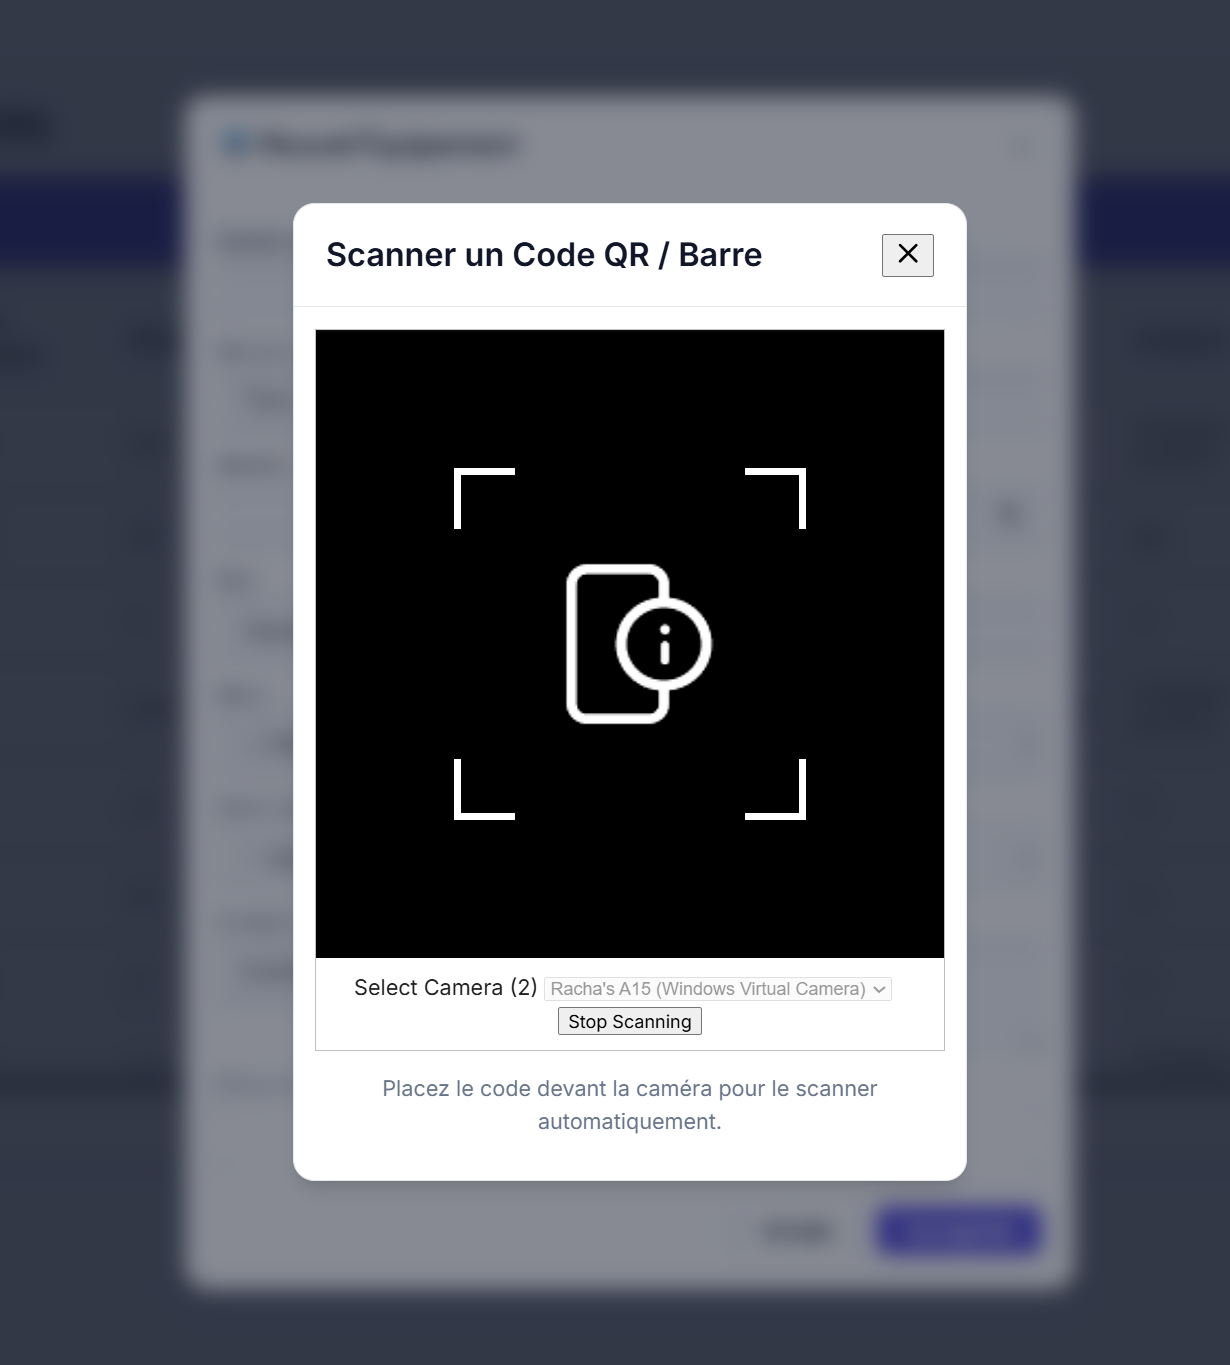
\includegraphics[width=1\textwidth]{chapter7/screens/ScanEaquimpentQR.png}
    \caption{Interface de scan mobile du QR code — accès instantané à la fiche d'un équipement sur le terrain}
    \label{fig:scan_qr}
\end{figure}

% =========================================================
\section{Optimisation des performances}
\label{sec:optimisation_performances}

La fiabilité fonctionnelle d'un système d'information ne saurait être dissociée de ses performances opérationnelles. Un tableau de bord dont le chargement dépasse plusieurs secondes, ou une API dont les temps de réponse se dégradent sous charge, peuvent nuire à l'adoption de la solution et à sa crédibilité auprès des utilisateurs. C'est pourquoi le Sprint 3 a accordé une attention particulière à l'optimisation des performances, tant côté backend que côté frontend.

\subsection*{Optimisations côté Backend (API Express)}

\begin{itemize}
    \item \textbf{Indexation standard des clés étrangères :} Sequelize crée automatiquement des index sur les colonnes de jointure (\texttt{equipementId}, \texttt{ticketId}, \texttt{TechnicienId}, etc.) lors de la synchronisation du schéma. Ces index optimisent les requêtes de jointure sur les tables à fort volume telles que \texttt{Ticket} et \texttt{Intervention} ;

    \item \textbf{Projection des attributs :} les endpoints de liste n'exposent que les attributs strictement nécessaires à l'affichage, via la clause \texttt{attributes} de Sequelize, réduisant le volume de données transférées ;

    \item \textbf{Agrégation SQL native :} les calculs de KPI sont réalisés directement au niveau de la base de données via des fonctions d'agrégation MySQL (\texttt{COUNT}, \texttt{AVG}, \texttt{SUM}, \texttt{GROUP BY}), évitant tout traitement itératif coûteux côté Node.js ;

    \item \textbf{Gestion asynchrone des notifications :} l'envoi des notifications FCM, implémenté dans une version simplifiée adaptée au cadre académique, est découplé du flux de traitement principal de la requête API via des promesses non bloquantes. La réponse HTTP est renvoyée au client dès la confirmation de la persistance en base, sans attendre la confirmation de livraison de la notification.
\end{itemize}

Ces optimisations restent adaptées au volume de données manipulé dans le cadre du prototype. À plus grande échelle, l'absence d'un cache applicatif dédié pour les statistiques les plus consultées et la génération de documents PDF/Excel côté serveur devront être réévaluées afin d'éviter les pics de charge lors d'exports volumineux.

\subsection*{Optimisations côté Frontend (React)}

\begin{itemize}
    \item \textbf{Mémorisation des calculs :} \texttt{useMemo} est appliqué aux composants de tableau de bord pour éviter les re-calculs inutiles lors des mises à jour partielles de l'état applicatif ;

    \item \textbf{Chargement asynchrone des données :} \texttt{@tanstack/react-query} gère le cycle de vie des requêtes API (mise en cache, rechargement automatique, états de chargement et d'erreur) sans bloquer l'interface utilisateur ;

    \item \textbf{Rendu conditionnel par rôle :} le composant \texttt{Dashboard.jsx} adapte dynamiquement son contenu (sections affichées, données chargées) en fonction du rôle de l'utilisateur authentifié, réduisant la charge mémoire du navigateur ;

    \item \textbf{Séparation des vues par rôle :} le routage de l'application charge uniquement les composants correspondant au rôle de l'utilisateur authentifié, réduisant à la fois la surface d'attaque côté sécurité et la charge mémoire du navigateur client.
\end{itemize}

% =========================================================
\section*{Conclusion}
\addcontentsline{toc}{section}{Conclusion}

Le Sprint 3 achève la construction d'un prototype fonctionnel de gestion de parc informatique cohérent, capable de couvrir les principales étapes du cycle de vie des actifs informatiques du SmartLab, de leur affectation à leur déclassement, en passant par le suivi opérationnel quotidien des incidents et des maintenances.

L'introduction de la dimension décisionnelle — tableaux de bord analytiques différenciés par profil, module de reporting exportable, indicateurs calculés en temps réel — permet à la plateforme de jouer le rôle d'outil de pilotage, et non plus seulement d'outil de saisie et de consultation. Le système de notification push, alimenté par Firebase FCM dans une version simplifiée adaptée au cadre académique, permet d’informer en temps réel les acteurs de la chaîne de maintenance des événements qui les concernent.

Les optimisations de performance réalisées au cours de cette itération indiquent la viabilité de l'architecture choisie dans le périmètre du prototype. Ces résultats ont été obtenus dans un environnement local de développement et doivent être considérés comme indicatifs. La plateforme constitue ainsi, dans le cadre de ce projet de fin d’études à une échelle locale, une contribution concrète à la modernisation de la gestion technique du patrimoine informatique de l'institution. Les performances estimées ainsi que la stabilité observée de l’architecture soutiennent la pertinence des choix techniques adoptés et ouvrent la voie à des évolutions futures du prototype dans un environnement universitaire.
